\chapter{Réalisation et mise en œuvre}
\label{ch:realisation}

Le chapitre précédent a permis de définir les principaux choix de conception de la plateforme : représentation multi-composante du document, règles explicites de classement, traitement automatisé sous contrôle humain, recherche hybride et génération augmentée par récupération, ainsi qu'une architecture modulaire intégrant les exigences de sécurité et de gouvernance. Le présent chapitre montre comment ces choix ont été concrètement mis en œuvre pour aboutir à une plateforme fonctionnelle déployée en environnement interne.

L'objectif n'est pas de reprendre les principes présentés précédemment ni de détailler chaque aspect du code, mais de montrer comment la conception s'est traduite dans la réalisation. Nous présentons ainsi l'environnement technique, l'implémentation du modèle documentaire et du pipeline de traitement, la recherche et l'assistance intelligente, puis les mécanismes de sécurité et les interfaces. Une attention particulière est également portée aux écarts entre les choix initialement conçus et leur mise en œuvre effective, ainsi qu'aux enseignements tirés des expérimentations menées sur les documents du \nomMinistere{}.

\section{Environnement technique de réalisation et d'exécution}

La réalisation s'appuie sur l'architecture présentée au chapitre précédent (figure~\ref{fig:archi-generale-conception}). Les traitements longs, notamment la reconnaissance du contenu, l'extraction et la vectorisation, sont isolés des interfaces et communiquent de manière asynchrone par l'intermédiaire d'un bus de messages. Ce découpage a guidé à la fois le choix des technologies et l'organisation du code.

Le backend est développé en Python et s'appuie sur FastAPI pour les services HTTP. Le frontend repose sur Next.js et constitue le point d'entrée des agents du ministère. La couche de données utilise PostgreSQL pour les métadonnées, les nœuds et les droits, ainsi que pgvector pour l'indexation des représentations vectorielles. Les fichiers sont conservés dans MinIO, tandis que RabbitMQ assure la communication asynchrone entre les différentes étapes du traitement. Redis complète cet ensemble pour la gestion du cache et de certains états d'exécution.

Les mécanismes de sécurité et d'exploitation sont intégrés au même environnement. Keycloak est utilisé pour l'authentification technique entre services et Vault pour la gestion des secrets de configuration. La supervision (Prometheus, Grafana, Loki, Vector) permet de suivre les files d'attente, les durées de traitement et les journaux, afin de détecter notamment un OCR bloqué ou un traitement trop long. Des tableaux de bord applicatifs, notamment avec Apache Superset, complètent le suivi d'activité destiné aux agents.

Le développement est réalisé localement avec Docker Compose. Les différents services, la base de données, le bus de messages et le stockage sont décrits dans une configuration versionnée, tandis que les paramètres d'exécution sont centralisés dans les fichiers d'environnement. L'environnement cible reprend le même assemblage de services dans un déploiement sur site (\textit{on-premise}) sur le réseau interne du ministère. En production, seuls les accès applicatifs nécessaires sont exposés ; les composants d'infrastructure restent isolés sur le réseau interne.

Les composants d'intelligence artificielle sont intégrés derrière des interfaces stables, afin de permettre l'évolution des modèles sans remettre en cause le reste du pipeline. La reconnaissance optique de caractères s'appuie sur Tesseract~5, retenu après comparaison interne (section~\ref{sec:eval-choix-briques}), avec la possibilité de recourir à un modèle de vision lorsque le texte extrait est insuffisant. L'audio et la vidéo sont transcrits à l'aide de Whisper. Les représentations vectorielles destinées à la recherche peuvent être produites par un modèle Sentence-BERT multilingue exécuté localement ou par un service d'embeddings externe, selon les contraintes de déploiement. La classification, le renommage et l'assistance conversationnelle sont assurés par le service de langage ; le modèle local retenu est Mistral~7B, exécuté via Ollama.

Cet environnement n'a pas vocation à constituer un inventaire exhaustif des dépendances du projet. Il permet surtout de montrer comment les différents éléments de l'architecture conçue au chapitre précédent ont été concrètement traduits en composants exécutables.

\section{Implémentation du modèle documentaire et du stockage}

Le modèle conçu au chapitre~\ref{ch:conception} distingue le fichier, l'enregistrement descriptif, le nœud d'exploration et l'index vectoriel. La réalisation conserve cette séparation : MinIO garde l'objet binaire ; PostgreSQL porte la description, l'arborescence, les droits et les vecteurs destinés à la recherche. Le nom de fichier n'est plus une clé ; un identifiant relie les composantes entre elles.

Les champs qui servent au classement et aux filtres (objet, type, source, sensibilité, dates, numéros) restent structurés. Un espace JSONB accueille ce qui n'entre pas dans ces colonnes, notamment le texte reconnu et des attributs propres à une famille documentaire. On évite ainsi deux écueils déjà rencontrés dans l'existant : un schéma trop rigide, et un index entièrement libre à la manière d'Excel.

Les types, expéditeurs et destinataires sont administrables. Le modèle de langage propose une valeur parmi ce vocabulaire, plutôt qu'un libellé inventé. Un même document peut être lié à plusieurs organismes, avec un principal pour le chemin. L'arborescence, elle, est un arbre de nœuds (dossier ou fichier). Le statut du nœud reste distinct du statut technique d'ingestion : \texttt{DRAFT} tant que la validation n'est pas confirmée, \texttt{VALIDATED} une fois le classement accepté, \texttt{ARCHIVED} pour la corbeille, et non pour des archives définitives. Le flux est matérialisé par les racines \texttt{Entrants}, \texttt{Sortants} et \texttt{Internes}. Le chemin conserve ensuite la règle expéditeur / type / année / mois.

Les fichiers arrivent d'abord dans une zone tampon MinIO, puis sont déplacés vers le chemin calculé après analyse. L'aperçu dans le navigateur passe par des liens temporaires, sans exposer le stockage. L'index de recherche est porté par les segments du document, et non par un vecteur unique attaché à la pièce entière : c'est ce qui permet le RAG par passages. Si un document est supprimé physiquement, ses segments le sont aussi.

La figure~\ref{fig:db-schema-postgres} traduit ce modèle en implémentation, sans inventaire de tables. Le fichier demeure dans MinIO (tampon, puis chemin calculé). PostgreSQL porte la description (champs structurés et JSONB), le nœud d'exploration et ses statuts, les référentiels, les droits, et les segments vectorisés destinés à la recherche.

\begin{figure}[H]
\centering
\begingroup
\shorthandoff{:;!?}
\usetikzlibrary{calc}
\resizebox{\textwidth}{!}{%
\begin{tikzpicture}[
  font=\sffamily,
  x=1cm, y=1cm,
  badge/.style={
    circle, minimum size=1.18cm,
    draw=black!30, line width=0.55pt
  },
  labfleche/.style={
    font=\sffamily\tiny, text=black!55, align=center, inner sep=1.5pt
  },
  lien/.style={
    -{Stealth[length=2.1mm, width=1.55mm]},
    draw=black!65, line width=0.7pt,
    dash pattern=on 1.15pt off 1.45pt
  }
]

% Pictogrammes simples (impression noir et blanc)
\tikzset{
  pics/icoDossier/.style={code={
    \fill[black!18] (-0.22,-0.14) rectangle (0.24,0.08);
    \fill[black!18] (-0.22,0.08) -- (-0.08,0.20) -- (0.06,0.08);
    \draw[black!55, line width=0.45pt] (-0.22,-0.14) rectangle (0.24,0.08);
    \draw[black!55, line width=0.45pt] (-0.22,0.08) -- (-0.08,0.20) -- (0.06,0.08);
  }},
  pics/icoPage/.style={code={
    \fill[white] (-0.16,-0.22) rectangle (0.16,0.22);
    \draw[black!55, line width=0.45pt] (-0.16,-0.22) rectangle (0.16,0.22);
    \draw[black!45, line width=0.4pt] (-0.08,0.10) -- (0.08,0.10);
    \draw[black!45, line width=0.4pt] (-0.08,0.00) -- (0.08,0.00);
    \draw[black!45, line width=0.4pt] (-0.08,-0.10) -- (0.04,-0.10);
  }},
  pics/icoListe/.style={code={
    \foreach \y in {0.12, 0.00, -0.12} {
      \fill[black!45] (-0.16,\y) circle (1.15pt);
      \draw[black!50, line width=0.45pt] (-0.08,\y) -- (0.18,\y);
    }
  }},
  pics/icoArbre/.style={code={
    \draw[black!55, line width=0.5pt] (0,0.16) -- (0,0.02);
    \draw[black!55, line width=0.5pt] (0,0.02) -- (-0.16,-0.14);
    \draw[black!55, line width=0.5pt] (0,0.02) -- (0.16,-0.14);
    \fill[black!20] (0,0.18) circle (3.1pt);
    \fill[black!20] (-0.16,-0.16) circle (2.5pt);
    \fill[black!20] (0.16,-0.16) circle (2.5pt);
    \draw[black!55, line width=0.4pt] (0,0.18) circle (3.1pt);
    \draw[black!55, line width=0.4pt] (-0.16,-0.16) circle (2.5pt);
    \draw[black!55, line width=0.4pt] (0.16,-0.16) circle (2.5pt);
  }},
  pics/icoClef/.style={code={
    \draw[black!55, line width=0.7pt] (0,0.10) circle (4.2pt);
    \fill[white] (0,0.10) circle (1.6pt);
    \draw[black!55, line width=0.7pt] (0,0.02) -- (0,-0.20);
    \draw[black!55, line width=0.7pt] (0,-0.08) -- (0.08,-0.08);
    \draw[black!55, line width=0.7pt] (0,-0.16) -- (0.08,-0.16);
  }},
  pics/icoSegments/.style={code={
    \fill[black!16] (-0.20,0.10) rectangle (0.20,0.20);
    \fill[black!22] (-0.20,-0.05) rectangle (0.20,0.05);
    \fill[black!16] (-0.20,-0.20) rectangle (0.20,-0.10);
    \draw[black!50, line width=0.4pt] (-0.20,0.10) rectangle (0.20,0.20);
    \draw[black!50, line width=0.4pt] (-0.20,-0.05) rectangle (0.20,0.05);
    \draw[black!50, line width=0.4pt] (-0.20,-0.20) rectangle (0.20,-0.10);
  }}
}

% ----- Niveau 1 : objet fichier (MinIO) -----
\node[font=\sffamily\bfseries\tiny, text=black!45, anchor=east]
  at (0.15, 8.55) {MinIO};

\node[badge, fill=green!12] (tampon) at (2.55, 8.55) {};
\pic at (tampon.center) {icoDossier};
\node[below=8pt of tampon, align=center] {%
  \sffamily\scriptsize\bfseries Zone tampon\\[-0.5pt]
  \sffamily\tiny\color{black!50}\texttt{buffer/}};

\node[badge, fill=green!12] (chemin) at (10.35, 8.55) {};
\pic at (chemin.center) {icoDossier};
\node[below=8pt of chemin, align=center] {%
  \sffamily\scriptsize\bfseries Chemin calculé\\[-0.5pt]
  \sffamily\tiny\color{black!50}expéditeur / type / année / mois};

\draw[lien] (tampon) -- (chemin)
  node[midway, above=3pt, labfleche] {déplacement après analyse};
\fill[black!75] (tampon.east) circle (1.55pt);
\fill[black!75] (chemin.west) circle (1.55pt);

% Bifurcation vers PostgreSQL
\coordinate (jonction) at ($(tampon.east)!0.50!(chemin.west)$);
\fill[black!75] (jonction) circle (1.7pt);

% ----- Niveau 2 : description et classement (PostgreSQL) -----
\node[font=\sffamily\bfseries\tiny, text=black!45, anchor=east]
  at (0.15, 4.15) {PostgreSQL};

\node[badge, fill=green!10] (ref) at (1.85, 4.15) {};
\pic at (ref.center) {icoListe};
\node[below=8pt of ref, align=center] {%
  \sffamily\scriptsize\bfseries Référentiels\\[-0.5pt]
  \sffamily\tiny\color{black!50}types, organismes};

\node[badge, fill=blue!10] (doc) at (6.45, 4.15) {};
\pic at (doc.center) {icoPage};
\node[below=8pt of doc, align=center] {%
  \sffamily\scriptsize\bfseries Document\\[-0.5pt]
  \sffamily\tiny\color{black!50}champs, JSONB, empreinte};

\node[badge, fill=blue!10] (noeud) at (10.35, 4.15) {};
\pic at (noeud.center) {icoArbre};
\node[below=8pt of noeud, align=center] {%
  \sffamily\scriptsize\bfseries Nœud\\[-0.5pt]
  \sffamily\tiny\color{black!50}DRAFT / VALIDATED / ARCHIVED};

\node[badge, fill=orange!12] (droits) at (14.15, 4.15) {};
\pic at (droits.center) {icoClef};
\node[below=8pt of droits, align=center] {%
  \sffamily\scriptsize\bfseries Droits\\[-0.5pt]
  \sffamily\tiny\color{black!50}rôles, ACL};

\draw[lien] (jonction) -- (doc.north)
  node[pos=0.42, labfleche, right=4pt, align=left] {référence\\de stockage};
\fill[black!75] (doc.north) circle (1.55pt);

\draw[lien] (ref) -- (doc)
  node[midway, above=3pt, labfleche] {vocabulaire};
\draw[lien] (doc) -- (noeud)
  node[midway, above=3pt, labfleche] {classement};
\draw[lien] (noeud) -- (droits)
  node[midway, above=3pt, labfleche] {accès};
\fill[black!75] (ref.east) circle (1.55pt);
\fill[black!75] (doc.west) circle (1.55pt);
\fill[black!75] (doc.east) circle (1.55pt);
\fill[black!75] (noeud.west) circle (1.55pt);
\fill[black!75] (noeud.east) circle (1.55pt);
\fill[black!75] (droits.west) circle (1.55pt);

% ----- Niveau 3 : index de recherche -----
\node[badge, fill=violet!12] (seg) at (6.45, 0.55) {};
\pic at (seg.center) {icoSegments};
\node[below=8pt of seg, align=center] {%
  \sffamily\scriptsize\bfseries Segments\\[-0.5pt]
  \sffamily\tiny\color{black!50}texte + vecteur (pgvector)};

\draw[lien] (doc.south) -- (seg.north)
  node[pos=0.48, labfleche, right=4pt, align=left] {index de\\recherche};
\fill[black!75] (doc.south) circle (1.55pt);
\fill[black!75] (seg.north) circle (1.55pt);

\end{tikzpicture}%
}
\endgroup
\vspace{0.12em}
\footnotesize Le fichier reste un objet MinIO ; PostgreSQL conserve sa référence de stockage ainsi que la description, le classement, l'index de recherche et les informations d'accès.

\caption{Traduction du modèle documentaire : fichier objet, enregistrement, nœud, segments et droits}
\label{fig:db-schema-postgres}
\end{figure}

\section{Réalisation du pipeline de traitement documentaire}

Le pipeline d'archivage enchaîne l'acquisition, la reconnaissance du contenu, l'analyse par modèle de langage, la détermination du classement à partir des métadonnées proposées, l'indexation et la validation humaine (figure~\ref{fig:flux-traitement}). Deux origines convergent vers la même entrée : le dossier surveillé des scanners, et le dépôt manuel depuis l'interface. La figure reprend la chaîne conçue au chapitre~\ref{ch:conception}, en y inscrivant ce qui a été effectivement implémenté : les files RabbitMQ, l'appel HTTP synchrone au modèle de langage, le nœud \texttt{DRAFT} et la confirmation humaine.

\begin{figure}[H]
\centering
\begingroup
\shorthandoff{:;!?}
\usetikzlibrary{calc}
\resizebox{\textwidth}{!}{%
\begin{tikzpicture}[
  font=\sffamily,
  x=1cm, y=1cm,
  etape/.style={
    circle, minimum size=1.48cm, line width=0.75pt
  },
  source/.style={
    circle, minimum size=1.18cm, line width=0.65pt,
    fill=cyan!14, draw=cyan!55!black!45
  },
  nom/.style={
    font=\sffamily\scriptsize\bfseries, text=black!80, align=center,
    inner sep=1pt
  },
  labfleche/.style={
    font=\sffamily\tiny, text=black!50, align=center, inner sep=1.2pt
  },
  carte/.style={
    rounded corners=2.5pt, align=left,
    font=\sffamily\tiny, inner xsep=6pt, inner ysep=4pt,
    text width=4.15cm, minimum height=0.62cm,
    line width=0.55pt
  },
  plein/.style={
    -{Stealth[length=2.2mm, width=1.6mm]},
    draw=black!45, line width=0.8pt
  },
  retour/.style={
    -{Stealth[length=2.2mm, width=1.6mm]},
    draw=magenta!55!black, line width=0.7pt,
    dash pattern=on 1.3pt off 1.5pt
  }
]

\tikzset{
  pics/icoInbox/.style={code={
    \draw[black!58, line width=0.7pt] (0,0.20) -- (0,0.02);
    \draw[black!58, line width=0.7pt] (-0.07,0.12) -- (0,0.20) -- (0.07,0.12);
    \draw[black!58, line width=0.55pt]
      (-0.20,-0.04) -- (-0.20,-0.20) -- (0.20,-0.20) -- (0.20,-0.04);
    \draw[black!58, line width=0.55pt] (-0.22,0.02) -- (0,-0.10) -- (0.22,0.02);
  }},
  pics/icoOeil/.style={code={
    \draw[black!58, line width=0.55pt] (0,0) ellipse (0.22cm and 0.12cm);
    \fill[black!58] (0,0) circle (3.3pt);
    \fill[white] (0.045,0.03) circle (1.15pt);
  }},
  pics/icoBulles/.style={code={
    \draw[black!58, line width=0.55pt] (-0.05,0.05) ellipse (0.16cm and 0.12cm);
    \draw[black!58, line width=0.55pt] (0.10,-0.07) ellipse (0.13cm and 0.10cm);
  }},
  pics/icoDossier/.style={code={
    \fill[green!25] (-0.20,-0.14) rectangle (0.22,0.06);
    \fill[green!25] (-0.20,0.06) -- (-0.08,0.18) -- (0.04,0.06);
    \draw[black!55, line width=0.5pt] (-0.20,-0.14) rectangle (0.22,0.06);
    \draw[black!55, line width=0.5pt] (-0.20,0.06) -- (-0.08,0.18) -- (0.04,0.06);
  }},
  pics/icoBarres/.style={code={
    \fill[orange!55!yellow!70] (-0.18,-0.16) rectangle (-0.08,0.02);
    \fill[orange!60!yellow!65] (-0.05,-0.16) rectangle (0.05,0.18);
    \fill[orange!50!yellow!75] (0.08,-0.16) rectangle (0.18,-0.04);
  }},
  pics/icoCheck/.style={code={
    \draw[orange!60!black, line width=1.15pt, line cap=round, line join=round]
      (-0.14,-0.02) -- (-0.03,-0.14) -- (0.18,0.14);
  }},
  pics/icoScan/.style={code={
    \draw[cyan!50!black, line width=0.5pt] (-0.16,-0.16) rectangle (0.16,0.16);
    \draw[cyan!45!black, line width=0.4pt] (-0.08,0.06) -- (0.08,0.06);
    \draw[cyan!45!black, line width=0.4pt] (-0.08,-0.02) -- (0.08,-0.02);
    \draw[cyan!50!black, line width=0.7pt] (-0.20,-0.20) -- (0.20,-0.20);
  }},
  pics/icoUpload/.style={code={
    \draw[cyan!50!black, line width=0.7pt] (0,0.18) -- (0,-0.04);
    \draw[cyan!50!black, line width=0.7pt] (-0.08,0.08) -- (0,0.18) -- (0.08,0.08);
    \draw[cyan!50!black, line width=0.5pt]
      (-0.16,-0.08) -- (-0.16,-0.18) -- (0.16,-0.18) -- (0.16,-0.08);
  }},
  pics/icoBranche/.style={code={
    \draw[white, line width=0.7pt] (0,0.16) -- (0,0.00);
    \draw[white, line width=0.7pt] (0,0.00) -- (-0.16,-0.14);
    \draw[white, line width=0.7pt] (0,0.00) -- (0.16,-0.14);
    \fill[white] (0,0.16) circle (1.7pt);
    \fill[white] (-0.16,-0.14) circle (1.5pt);
    \fill[white] (0.16,-0.14) circle (1.5pt);
  }},
  pics/icoVision/.style={code={
    \draw[magenta!60!black, line width=0.55pt] (0,0) ellipse (0.20cm and 0.11cm);
    \fill[magenta!60!black] (0,0) circle (2.9pt);
    \fill[white] (0.04,0.025) circle (1pt);
  }}
}

% ----- Sources -----
\node[source] (scan) at (1.15, 8.15) {};
\pic at (scan.center) {icoScan};
\node[nom, above=18pt of scan] {Scanners};
\node[font=\sffamily\tiny, text=black!50, above=7pt of scan] {scan-listener};

\node[source] (upload) at (1.15, 5.05) {};
\pic at (upload.center) {icoUpload};
\node[nom, above=18pt of upload] {Dépôt manuel};
\node[font=\sffamily\tiny, text=black!50, above=7pt of upload] {\texttt{POST /upload}};

% ----- Chaîne principale -----
\node[etape, fill=blue!13, draw=blue!55!black!50] (a1) at (4.05, 6.60) {};
\pic at (a1.center) {icoInbox};
\node[nom, above=10pt of a1] {Acquisition};

\node[etape, fill=cyan!16, draw=cyan!55!black!45] (a2) at (6.70, 6.60) {};
\pic at (a2.center) {icoOeil};
\node[nom, above=10pt of a2] {Reconnaissance};

\node[etape, fill=purple!14, draw=purple!50!black!45] (a3) at (9.35, 6.60) {};
\pic at (a3.center) {icoBulles};
\node[nom, above=10pt of a3] {Analyse LLM};

\node[etape, fill=green!14, draw=green!50!black!45] (a4) at (12.00, 6.60) {};
\pic at (a4.center) {icoDossier};
\node[nom, above=10pt of a4] {Classement};
\node[font=\sffamily\tiny, text=green!40!black, below=8pt of a4] {\texttt{DRAFT}};

\node[etape, fill=yellow!22!orange!12, draw=orange!50!black!40] (a5) at (14.65, 6.60) {};
\pic at (a5.center) {icoBarres};
\node[nom, above=10pt of a5] {Indexation};

\node[etape, fill=orange!22, draw=orange!60!black!45] (a6) at (17.30, 6.60) {};
\pic at (a6.center) {icoCheck};
\node[nom, above=10pt of a6] {Validation};
\node[font=\sffamily\tiny, text=orange!50!black, below=8pt of a6] {\texttt{VALIDATED}};

\draw[plein] (scan.east) -- (a1.west);
\draw[plein] (upload.east) -- (a1.west);
\draw[plein] (a1) -- (a2);
\draw[plein] (a2) -- (a3);
\draw[plein] (a3) -- (a4);
\draw[plein] (a4) -- (a5);
\draw[plein] (a5) -- (a6);

% ----- Reconnaissance selon le support -----
\node[
  rounded corners=5pt, fill=cyan!6, draw=cyan!35!black!30,
  dashed, line width=0.65pt,
  minimum width=13.35cm, minimum height=2.55cm,
  anchor=south west
] at (4.85, 0.55) {};

\node[etape, minimum size=1.32cm, fill=cyan!65!black, draw=none] (br) at (6.70, 2.00) {};
\pic at (br.center) {icoBranche};
\node[nom, below=8pt of br] {Selon le support};

\draw[plein, draw=cyan!50!black] (a2.south) -- (br.north);

\node[carte, fill=green!12, draw=green!45!black!40] (cnat) at (10.55, 2.72)
  {\textbf{Bureautique, texte}\\[-1pt]extracteur selon le format};
\node[carte, fill=blue!12, draw=blue!45!black!40] (cocr) at (10.55, 2.00)
  {\textbf{PDF, image}\\[-1pt]Tesseract};
\node[carte, fill=purple!12, draw=purple!45!black!40] (cwsp) at (10.55, 1.28)
  {\textbf{Audio, vidéo}\\[-1pt]Whisper};

\draw[plein, draw=cyan!50!black] (br.east) -- (cocr.west);

\node[etape, minimum size=1.32cm, fill=magenta!14, draw=magenta!50!black!40] (vis) at (15.35, 2.00) {};
\pic at (vis.center) {icoVision};
\node[below=8pt of vis, align=center] {%
  \sffamily\scriptsize\bfseries Repli vision\\[-0.4pt]
  \sffamily\tiny\color{black!50}si texte non exploitable};

\draw[plein, draw=magenta!55!black] (cocr.east) -- (vis.west);

\draw[retour] (vis.north) -- ++(0, 1.35) -| (a3.south)
  node[pos=0.16, labfleche, right=2pt] {contenu retenu};

\end{tikzpicture}%
}
\endgroup
\vspace{0.12em}
\footnotesize \textbf{Légende :} trait plein = enchaînement du pipeline ; pointillé = retour après reconnaissance, y compris le repli vision.

\caption{Pipeline réalisé : de l'arrivée du fichier à la validation, avec reconnaissance selon le support et nœud \texttt{DRAFT}}
\label{fig:flux-traitement}
\end{figure}

\subsection{Acquisition et gestion des fichiers}

Le scan-listener surveille un répertoire partagé. Lorsqu'un fichier apparaît et n'est plus en cours d'écriture, il est soumis au service d'upload. En cas d'échec persistant, le fichier est déplacé vers un répertoire d'erreur, avec une copie de sauvegarde, afin de ne pas bloquer la file des scans suivants. L'upload manuel suit le même contrat : \texttt{POST /upload} (multipart). Le fichier est lu, son empreinte SHA-256 est calculée, puis l'objet est écrit dans le tampon MinIO. Un message \texttt{document.uploaded} est alors publié sur RabbitMQ, portant l'identifiant du document et le chemin de stockage. L'enregistrement PostgreSQL est créé dans la foulée, avec cette référence et cette empreinte, afin que le suivi et les étapes suivantes puissent s'y rattacher. La reconnaissance en aval s'appuie ainsi sur un objet déjà disponible ; elle n'est pas déclenchée sur un dépôt incomplet. La requête s'achève à ce stade ; la reconnaissance du contenu se poursuit ensuite en arrière-plan. L'agent du ministère peut donc continuer à travailler sans attendre la fin de l'OCR.

L'empreinte est conservée avec l'enregistrement. Elle n'interrompt pas la file d'ingestion : le service d'upload enregistre le fichier même si un autre fichier possédant la même empreinte SHA-256 existe déjà. En revanche, lors d'un dépôt depuis l'interface, une comparaison peut signaler à l'agent qu'un fichier binaire identique selon cette empreinte est déjà présent, sans révéler un document hors de son périmètre. L'écran de vérification, présenté plus loin, reprend ce mécanisme.

\subsection{Reconnaissance du contenu selon le support}

Le service OCR consomme \texttt{document.uploaded}, récupère l'objet et oriente le traitement selon le type de contenu, plutôt que d'appliquer un unique moteur à tous les fichiers.

Les fichiers bureautiques et les fichiers textuels (documents Word, tableurs, présentations, CSV, etc.) sont traités par des extracteurs adaptés à leur format, éventuellement complétés par un extracteur structuré lorsque le résultat est trop pauvre. Les images sont soumises à Tesseract, moteur d'OCR libre présenté par \citer{smith2007}{Smith (2007)}, en français et en anglais. Tous les PDF, y compris ceux nativement numériques, suivent le même chemin : chaque page est rendue en image, puis reconnue par Tesseract. Aucune extraction de la couche texte du PDF n'est utilisée dans cette version. L'audio est transcrit par Whisper (modèle \texttt{small}, langue française par défaut). Pour la vidéo, la piste sonore est d'abord extraite, puis transcrite de la même manière ; si cette transcription n'est pas exploitable, une image clé peut alimenter une analyse visuelle complémentaire.

La conception prévoyait une lecture directe de la couche texte lorsque le PDF en porte une. Cette voie n'a pas été retenue : un seul pipeline OCR permet de traiter de manière uniforme un fonds où scans et fichiers nés numériques coexistent.

Quel que soit le canal, une heuristique (longueur, lettres, ratio alphanumérique) juge si le texte est exploitable. Un résultat vide, trop court ou trop bruité ne signifie pas que le document est vide. Lorsqu'une page contient encore du texte difficile à extraire (formulaire manuscrit, tampon, scan peu contrasté), un modèle de vision tente de le transcrire. Lorsqu'il s'agit surtout d'une image, d'un schéma ou d'une capture, le même repli produit une description sémantique. Dans les deux cas, le classifieur ne reçoit qu'une représentation textuelle, transcription ou description, plutôt que le bruit d'un OCR vide.

Le texte retenu, la méthode employée et, le cas échéant, une légende ou des étiquettes visuelles sont persistés dans les métadonnées JSONB. Un message \texttt{ocr.completed} déclenche alors l'extraction.

\subsection{Analyse par LLM, métadonnées, renommage et classement}

L'extraction-service consomme \texttt{ocr.completed} et appelle de manière synchrone le language-model-service (\texttt{POST /classify-and-rename}) : le service attend la réponse HTTP avant de poursuivre. Le prompt fournit le texte (borné, afin de rester dans une fenêtre raisonnable), la liste des types documentaires actifs et les consignes de nommage du ministère. Le modèle propose l'expéditeur, le destinataire, les numéros, l'objet, le type, la sensibilité (\texttt{public}, \texttt{interne}, \texttt{confidentiel}, \texttt{secret}), la date d'arrivée et la source (entrant, sortant ou interne). Ces propositions sont écrites en base ; elles ne valident pas l'archivage.

Le renommage suit la nomenclature déjà attendue : \texttt{[Expéditeur] - [Numéro] - [Objet]}, avec \texttt{0000} lorsque le numéro interne est introuvable. Le chemin n'est pas généré par le modèle de langage. À partir des métadonnées proposées, l'application calcule le classement, par exemple :

\begin{center}
\texttt{Entrants/presidence-republique/courriel/2026/03/[PRESIDENCE] - [0000] - [Objet].pdf}
\end{center}

L'objet MinIO est copié vers cette clé ; le nœud d'exploration est créé ou mis à jour en \texttt{DRAFT}. Si la copie échoue, les métadonnées restent enregistrées tandis que le fichier demeure dans la zone tampon ; l'erreur est journalisée : le traitement métier n'est pas perdu pour autant. Un traitement à nouveau (\texttt{reprocess}) permet de relancer la chaîne sur un document déjà présent.

\subsection{Embeddings et validation humaine}

Une fois le texte et les champs métier disponibles, le contenu est découpé en passages d'environ 2\,000 caractères, avec un chevauchement de 400 caractères, afin de préserver une continuité contextuelle entre passages tout en limitant leur taille. Les champs métier (objet, expéditeur, type, destinataire, numéro interne) sont indexés à part, comme unités distinctes des segments de contenu. Chaque unité est vectorisée et insérée dans \texttt{document\_chunks}. Les documents en \texttt{DRAFT} peuvent être indexés ; l'accès aux résultats de recherche, et aux extraits transmis au modèle de langage, est ensuite filtré par le statut du nœud, les ACL et la sensibilité.

La confirmation reste humaine : sans validation, le nœud demeure en \texttt{DRAFT}. C'est le principe d'assistance contrôlée. Dans l'espace de traitement, le validateur voit le fichier, le texte extrait, les champs proposés et le classement calculé. Il peut corriger l'expéditeur, l'objet, la source ou le type, puis valider. La validation passe le nœud en \texttt{VALIDATED}, fige la date de validation et, si nécessaire, reclasse le fichier lorsque la date d'arrivée ou la source a été corrigée. Pour les archives anciennes, cinq agents ont participé au contrôle de ces propositions, compte tenu de la sensibilité et de la difficulté particulières de ce corpus.

\subsection{Erreurs et reprises}

L'asynchronisme sert aussi la reprise. La remise en file (\texttt{requeue}) n'est utilisée que pour une erreur transitoire, par exemple une indisponibilité momentanée. Une erreur définitive n'est jamais remise automatiquement : le message est retiré de la file, afin d'éviter une boucle infinie. Le scan-listener isole les fichiers en échec dans un répertoire d'erreur, avec une copie de sauvegarde. Les files \texttt{vector.reindex} et \texttt{acl.recompute} permettent de reconstruire l'index ou les droits sans réingérer le binaire. L'agent, pendant ce temps, continue de travailler.

\section{Réalisation de la recherche et de l'assistance intelligente}

La conception du RAG (figure~\ref{fig:rag-pipeline}) est implémentée dans le routing-service, en s'appuyant sur l'extraction-service pour la recherche filtrée et sur le language-model-service pour la génération. Le corpus interrogé par défaut est celui des nœuds \texttt{VALIDATED} ; les pièces en brouillon et celles de la corbeille n'entrent pas dans le contexte du modèle.

\subsection{Indexation, recherche hybride et fusion}

Les segments de contenu et les champs métier produits par le pipeline de traitement sont enregistrés dans PostgreSQL avec leur représentation vectorielle dans \texttt{pgvector}. Le modèle d'embedding est configurable selon l'environnement d'exécution. La configuration locale repose sur le modèle Sentence-BERT multilingue \texttt{paraphrase-multilingual-MiniLM-L12-v2}, produisant des vecteurs de 384 dimensions \citp{reimers2019}{Reimers et Gurevych, 2019}, tandis qu'un service d'embeddings externe peut être utilisé avec des vecteurs de 1024 dimensions. Pour chaque index, les requêtes sont vectorisées avec le même modèle que celui utilisé pour les documents indexés.

Lorsqu'une requête est soumise, le filtrage de sécurité détermine d'abord l'ensemble $D$ des documents autorisés. Trois listes de candidats sont ensuite construites sur $D$, selon les méthodes $\mathcal{M}$ du chapitre~\ref{ch:conception}. La première, $L_{\mathrm{dense}}$, est une récupération dense au sens du Dense Passage Retrieval : similarité entre l'embedding de la requête et ceux des unités indexées (segments de contenu et champs métier) \citp{karpukhin2020}{Karpukhin et al., 2020}. La deuxième, $L_{\mathrm{lex}}$, exploite la correspondance lexicale dans le texte des segments, notamment par recherche de sous-chaînes accélérée par l'extension \texttt{pg\_trgm} de PostgreSQL ; la recherche plein texte n'est pas appliquée directement aux segments. La troisième, $L_{\mathrm{doc}}$, combine une recherche plein texte en français (\texttt{tsvector}, \texttt{plainto\_tsquery}) et des correspondances de sous-chaînes sur des attributs tels que le nom du fichier, l'objet, les tags et la description.

Cette troisième liste constitue une source de candidats indépendante et ne se limite donc pas à filtrer les résultats issus des deux autres. Des filtres optionnels portant notamment sur le type documentaire ou les dates peuvent toutefois restreindre les trois branches avant leur fusion. Les listes sont combinées par Reciprocal Rank Fusion selon l'équation~\eqref{eq:rrf}, avec $k=60$ \citp{cormack2009}{Cormack, Clarke et Buettcher, 2009}. Cette constante est celle de la configuration classique ; elle n'a pas été calibrée sur le jeu de test présenté plus bas. Aucune pondération supplémentaire n'est appliquée ($w_{m} = 1$). Un réordonnancement lexical léger n'intervient qu'après cette fusion.

L'expansion lexicale de la requête (synonymes du vocabulaire métier, par exemple entre \og arrêté\fg{}, \og décret\fg{} et \og circulaire\fg{}, ou entre \og marché\fg{} et \og offres\fg{}) et une seconde passe (seuils assouplis, éventuellement reformulation) sont implémentées comme mécanismes de secours lorsque la première récupération ne fournit pas d'extraits suffisants \citp{azad2019}{Azad et Deepak, 2019}. Elles n'ont pas été isolées dans l'évaluation de ce chapitre : les métriques rapportées caractérisent le pipeline tel qu'il s'exécute, et non la contribution propre de ces secours.

L'interface de recherche conversationnelle utilise par défaut huit extraits. Les seuils de similarité sont configurables et ne servent pas à interpréter les scores RRF, qui mesurent un rang fusionné plutôt qu'une similarité cosinus. Avant transmission au modèle, chaque passage est réduit de façon extractive : les phrases les plus proches de la requête sont retenues, puis la longueur est bornée (environ 800 caractères). Cette réduction vise à contenir la taille du prompt ; ce n'est pas une méthode nommée de \textit{context compression}. Le constat de \citer{liu2024}{Liu et al. (2024)} sur la dégradation des modèles face à un contexte trop long motive l'objectif, sans valider expérimentalement cet algorithme sur notre corpus. Une règle de diversification évite qu'un même document monopolise les $N$ extraits.

\subsection{Filtrage, génération et sources}

Avant la récupération des passages, le système applique les contraintes de sécurité associées à l'utilisateur courant. Elles portent notamment sur le niveau de sensibilité autorisé (MAC), le statut des nœuds, les droits d'accès définis par les ACL et, le cas échéant, la restriction à un document explicitement ouvert. Ces contraintes déterminent l'ensemble des documents susceptibles d'alimenter la recherche et empêchent qu'un contenu non autorisé soit transmis au modèle de langage (\citer{namer2024}{Namer et al., 2024} ; \citer{owasp2025}{OWASP, 2025}). Un document encore en \texttt{DRAFT} ou placé dans la corbeille est ainsi exclu de l'assistance par défaut.

Après filtrage et récupération, le modèle de langage reçoit l'historique pertinent de la conversation, les passages sélectionnés et une consigne précisant que la réponse doit s'appuyer sur ce contexte. Lorsque les éléments récupérés ne permettent pas de répondre à la question, le modèle doit signaler l'insuffisance de l'information disponible plutôt que de compléter la réponse par une information non présente dans les sources \citp{nist2024}{NIST, 2024}.

Chaque passage transmis au modèle conserve une référence vers le document et son emplacement dans celui-ci. La réponse peut ainsi être accompagnée de sources permettant à l'agent de retrouver et d'ouvrir la pièce correspondante. Cette traçabilité permet de relier la réponse générée aux documents effectivement utilisés et constitue un élément essentiel de l'assistance documentaire fondée sur la récupération, au-delà de la seule génération de texte \citp{lewis2020}{Lewis et al., 2020}.

\section{Mise en œuvre de la sécurité et de la gouvernance}

La sécurité mise en œuvre repose sur plusieurs couches complémentaires, conformément aux principes définis lors de la conception : authentification des utilisateurs, authentification technique entre services, contrôle d'accès par rôles (RBAC), contrôle d'accès aux nœuds (ACL), limitation par niveau de sensibilité, cloisonnement du stockage et journalisation des opérations.

Les utilisateurs s'authentifient via NextAuth, tandis que les rôles et les permissions sont enregistrés dans PostgreSQL. Les trois profils de base, à savoir validateur, administrateur et lecteur, correspondent à des compositions de permissions pouvant être modifiées sans redéploiement de l'application. Un rôle peut également être associé à un plafond de sensibilité. Lorsqu'un document dépasse ce niveau, il est exclu des ressources accessibles à l'utilisateur, y compris dans les résultats de recherche et les interactions avec l'assistant.

Les ACL définissent des autorisations \texttt{ALLOW} associées à un nœud pour un utilisateur, un groupe ou un rôle. Ces autorisations sont héritées par les descendants. Lorsqu'une autorisation locale et une autorisation héritée concernent le même principal, la règle locale est prioritaire. La version réalisée ne prévoit pas de règle \texttt{DENY} explicite. Un fichier peut être placé en mode restreint, dans lequel son accès est limité notamment à son déposant jusqu'à son partage, ou en mode public pour les utilisateurs authentifiés. Les documents provenant du \texttt{scan-listener} sont, selon la politique retenue, accessibles aux utilisateurs de l'organisation, puisqu'ils correspondent au flux d'archives collectives. Les dépôts effectués depuis l'interface restent, par défaut, restreints. Un partage direct sur un fichier suffit à autoriser son accès, même lorsque son dossier parent n'est pas visible par l'utilisateur. Une ressource pour laquelle l'utilisateur ne dispose d'aucun droit est traitée comme inexistante, afin de ne pas révéler son existence.

L'authentification des services repose sur Keycloak, distinctement de l'authentification des utilisateurs. Les communications entre services utilisent des jetons obtenus selon le mécanisme \texttt{client-credentials}, dans un realm dédié et avec des portées correspondant aux opérations autorisées, telles que \texttt{ged:lm:classify}, \texttt{ged:upload:write} ou \texttt{ged:minio:presign}. L'\texttt{extraction-service} utilise ainsi son identité technique pour appeler le service de classification, tandis que les services autorisés peuvent effectuer les opérations de stockage nécessaires. Vault fournit les secrets aux conteneurs au démarrage au moyen d'AppRole, ce qui évite de les conserver directement dans les images. MinIO est utilisé comme stockage objet et non comme partage de fichiers. Les comptes techniques disposent de permissions limitées et les utilisateurs finaux n'accèdent pas directement au stockage : l'accès passe par les API de la plateforme, après vérification des autorisations.

L'empreinte SHA-256 est calculée lors de l'upload et conservée dans \texttt{documents.file\_hash}, avec un index dédié. L'écran de vérification permet de soumettre un fichier afin de rechercher une éventuelle correspondance. Lorsqu'un doublon est identifié dans le périmètre accessible à l'utilisateur, les informations du document concerné peuvent être affichées. Lorsqu'une correspondance existe en dehors de ce périmètre, aucune information ne permet d'en révéler l'existence. Cette règle permet de combiner détection des doublons et cloisonnement des informations.

Enfin, les opérations importantes, notamment la validation, la modification des métadonnées, les changements de droits et les opérations d'administration, sont enregistrées dans \texttt{document\_events} avec l'utilisateur concerné, l'horodatage et le document associé. Cette journalisation permet de distinguer les propositions produites automatiquement par le pipeline des décisions prises par les agents et fournit ainsi un mécanisme de traçabilité des opérations documentaires.

\section{Réalisation des interfaces}

Les interfaces réalisées traduisent les principaux parcours du travail documentaire présentés lors de la conception. Leur organisation privilégie les actions effectivement disponibles pour l'utilisateur, tandis que les fonctionnalités accessibles sont déterminées par les permissions qui lui sont attribuées.

Le parcours de traitement et de validation constitue le premier espace central de la plateforme. Il permet de suivre les documents en cours d'analyse, de consulter le fichier et le contenu extrait, puis d'examiner les métadonnées et le classement proposés (figure~\ref{fig:ui-traitement-validation}). Le validateur peut corriger les informations nécessaires avant de confirmer l'archivage.

\begin{figure}[H]
\centering
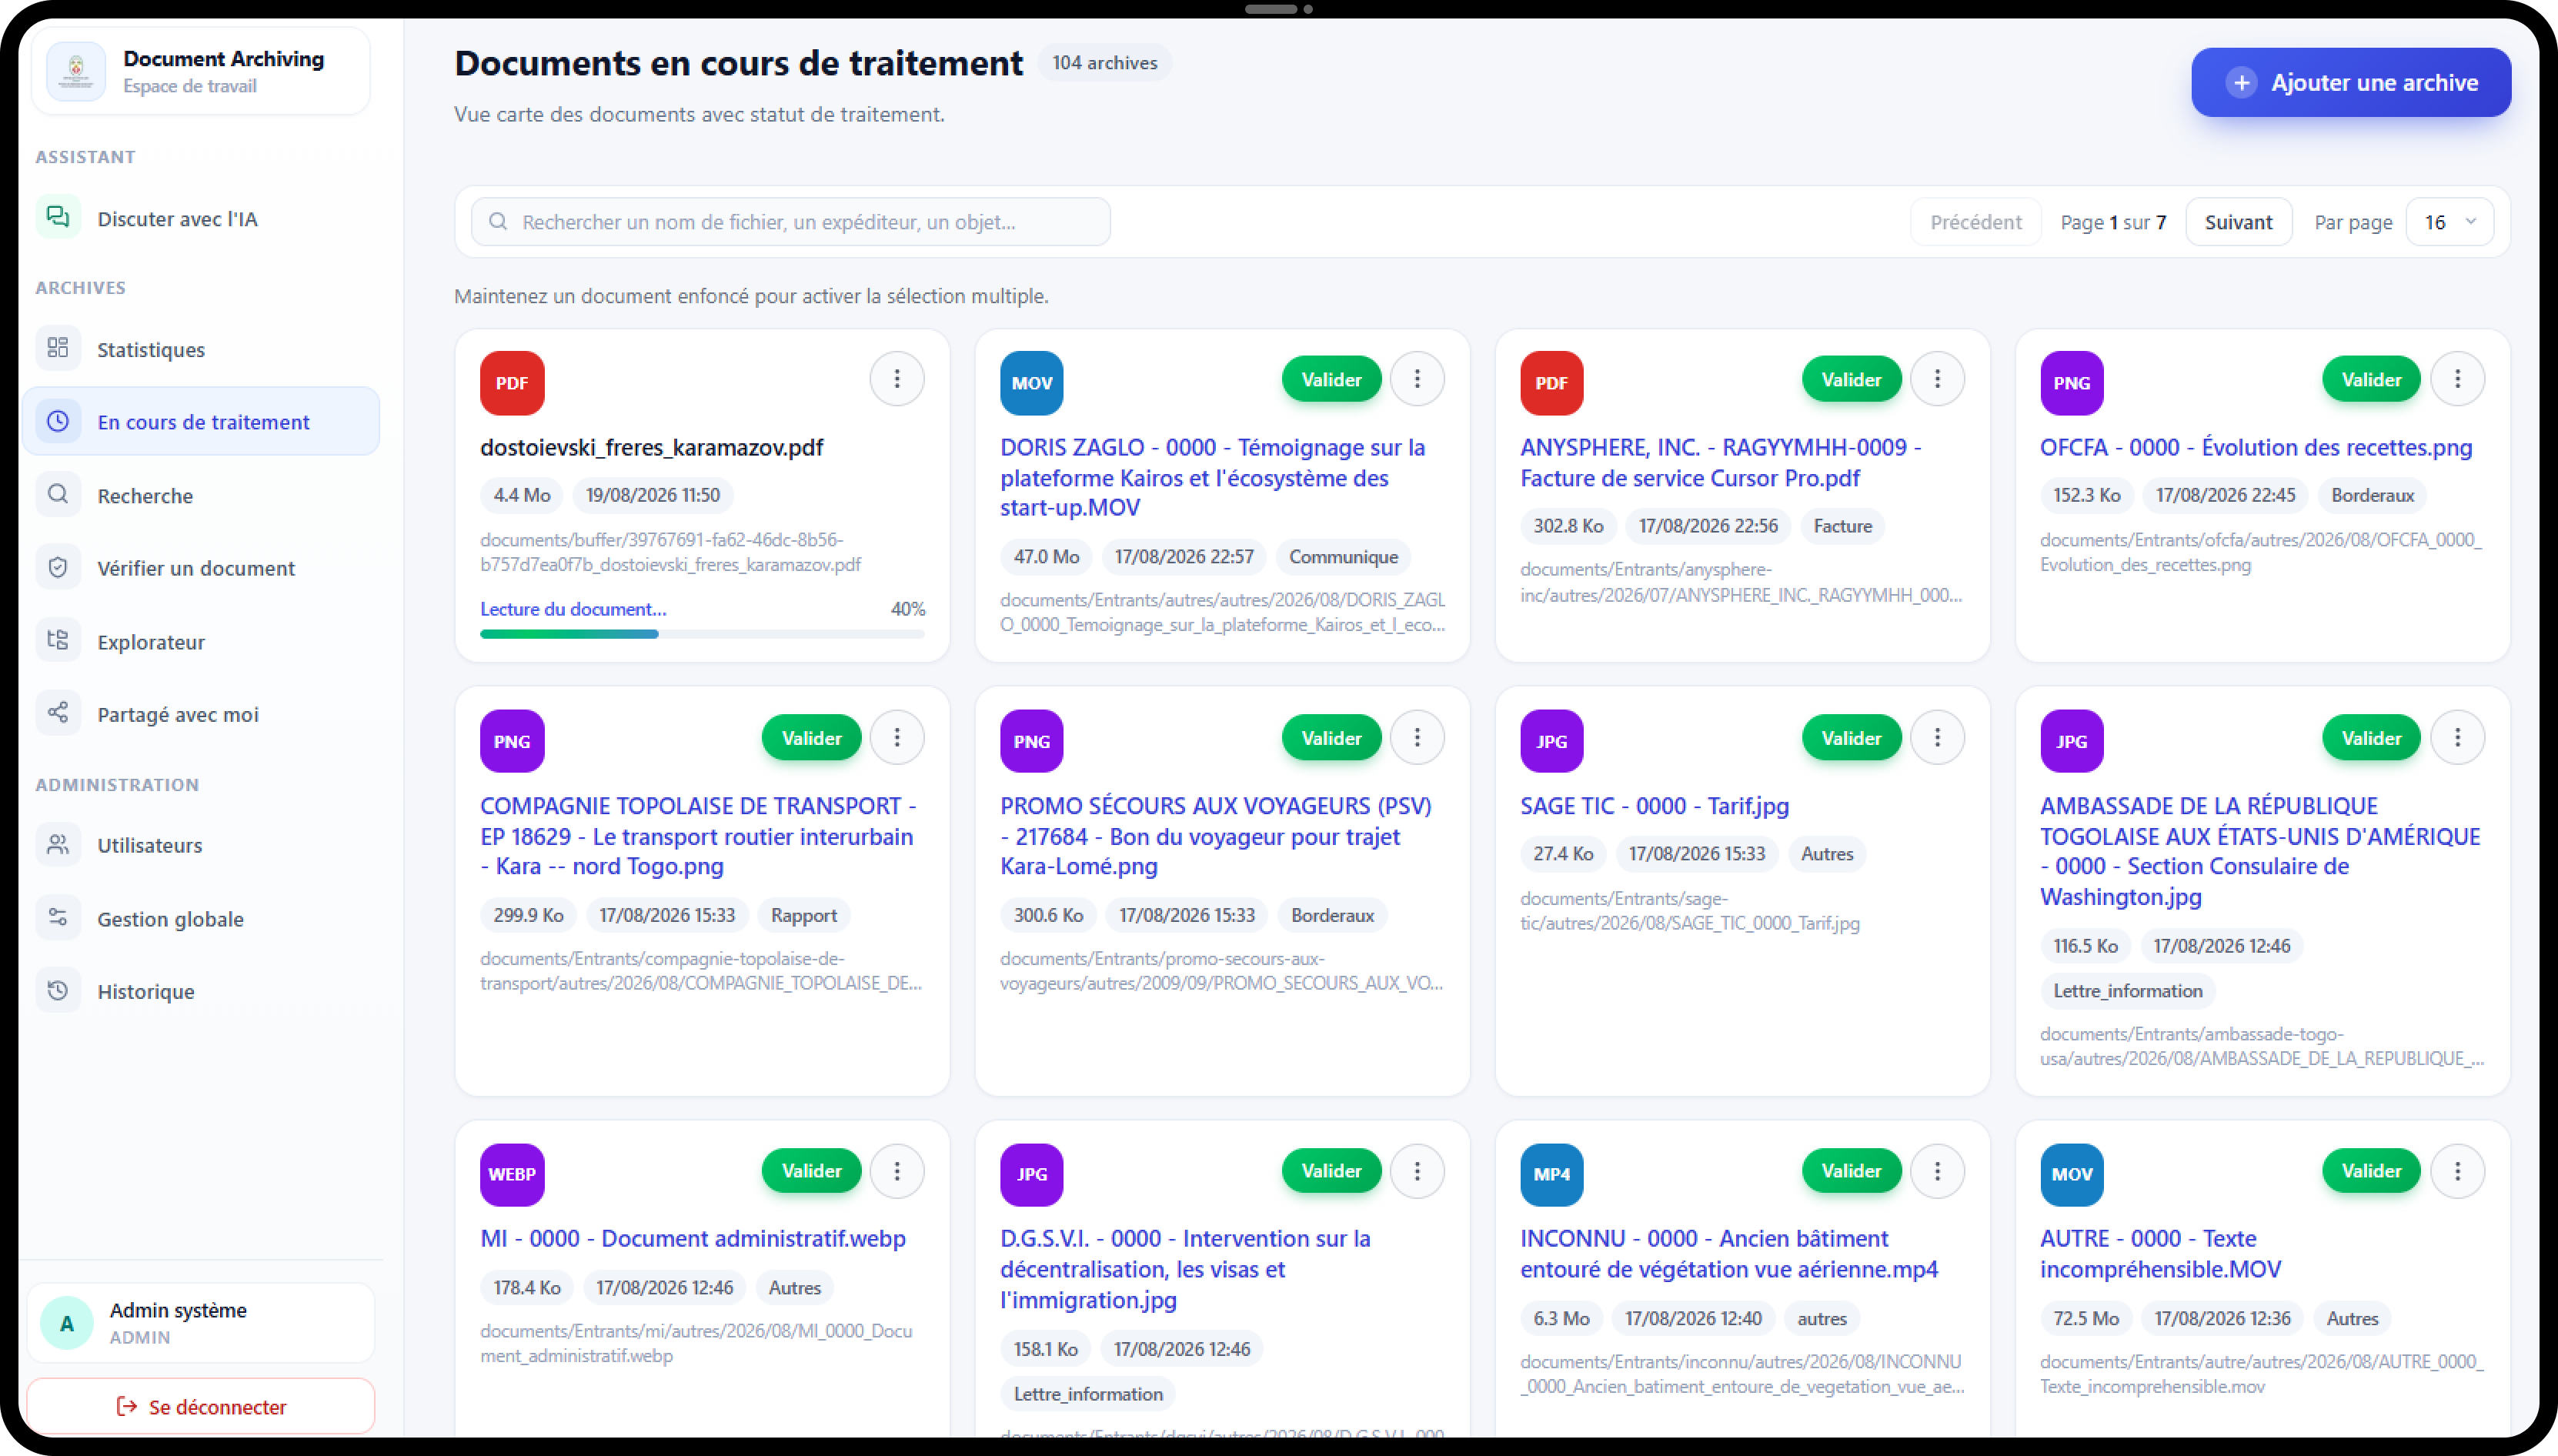
\includegraphics[width=0.98\textwidth]{images/screens/Traitement_documents.png}
\caption{Interface de traitement et de validation d'un document}
\label{fig:ui-traitement-validation}
\end{figure}

L'interface d'exploration documentaire reprend l'organisation retenue pour le classement, avec les niveaux Entrants, Sortants ou Internes, puis expéditeur, type documentaire, année et mois (figure~\ref{fig:ui-exploration}). Elle permet ainsi de retrouver les documents selon une logique proche de l'arborescence définie lors de la conception.

\begin{figure}[H]
\centering
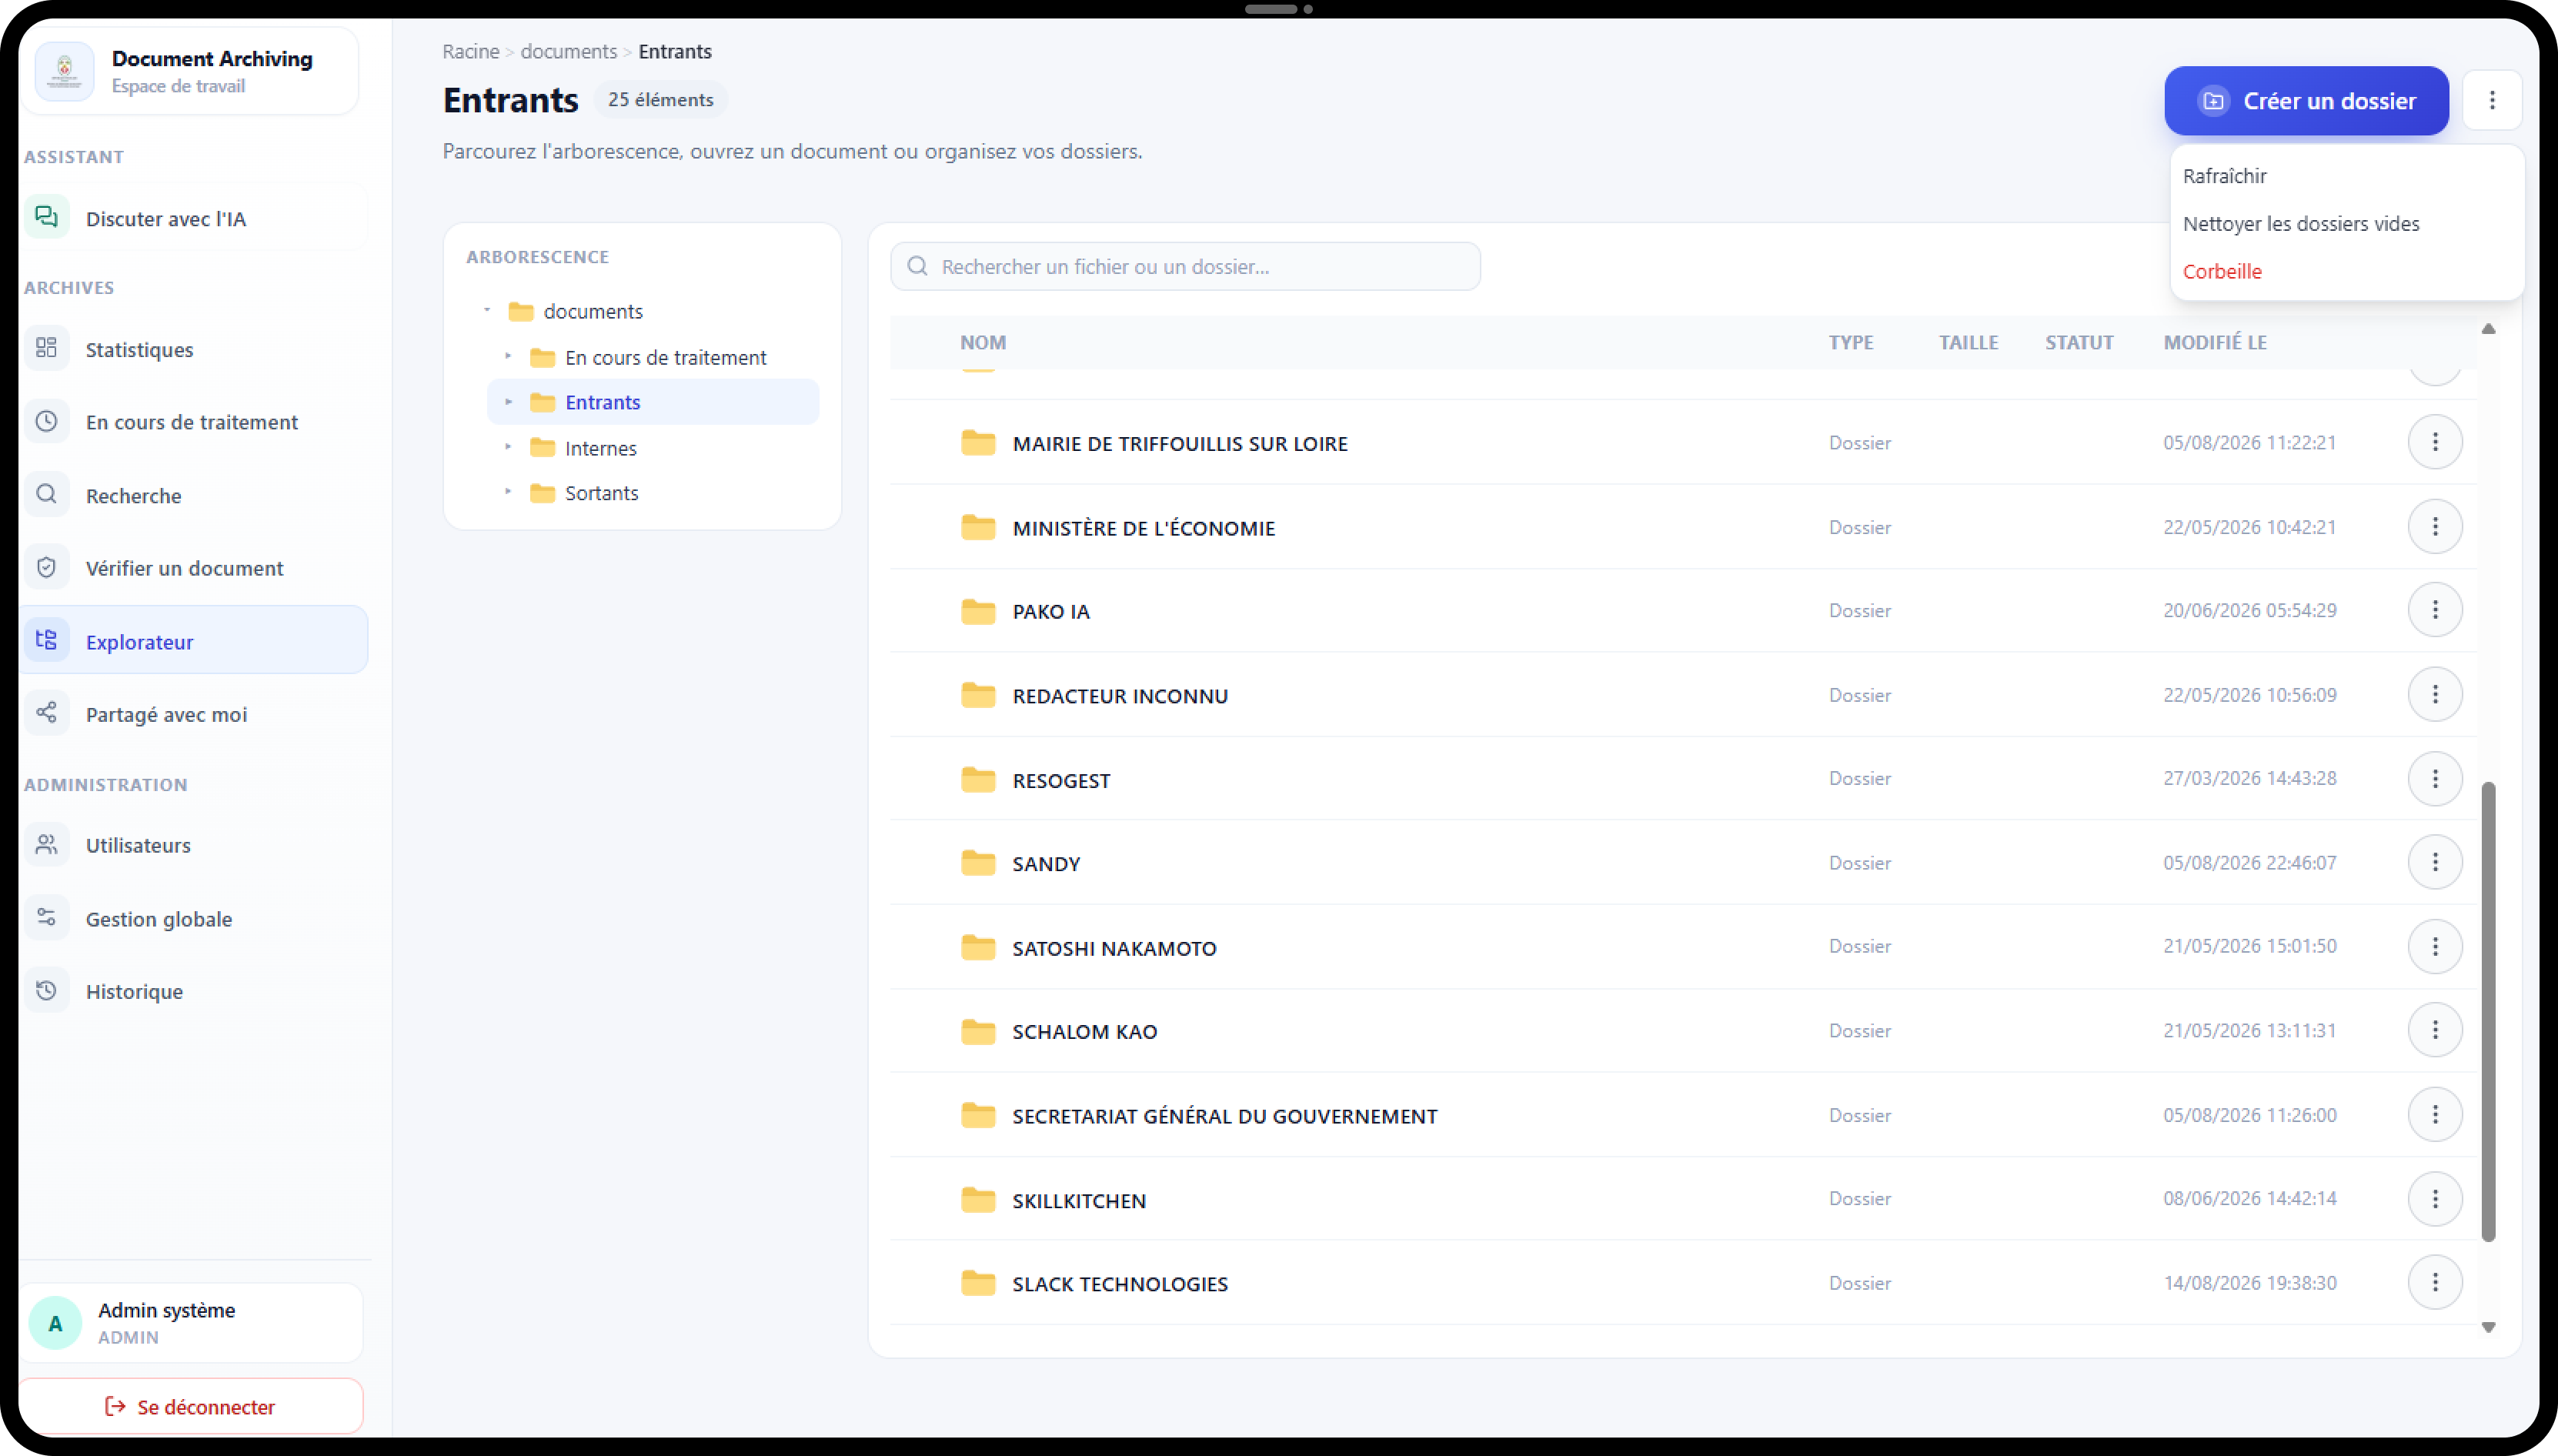
\includegraphics[width=0.98\textwidth]{images/screens/exploration_arborescence.png}
\caption{Interface d'exploration du fonds documentaire}
\label{fig:ui-exploration}
\end{figure}

La recherche et l'assistance intelligente constituent le second parcours majeur. L'utilisateur peut effectuer une recherche à partir de mots-clés et de filtres, ou formuler directement une question en langage naturel. Dans ce dernier cas, la réponse générée est accompagnée des sources utilisées, qui peuvent être ouvertes pour vérifier l'information fournie (figure~\ref{fig:ui-assistant}).

\begin{figure}[H]
\centering
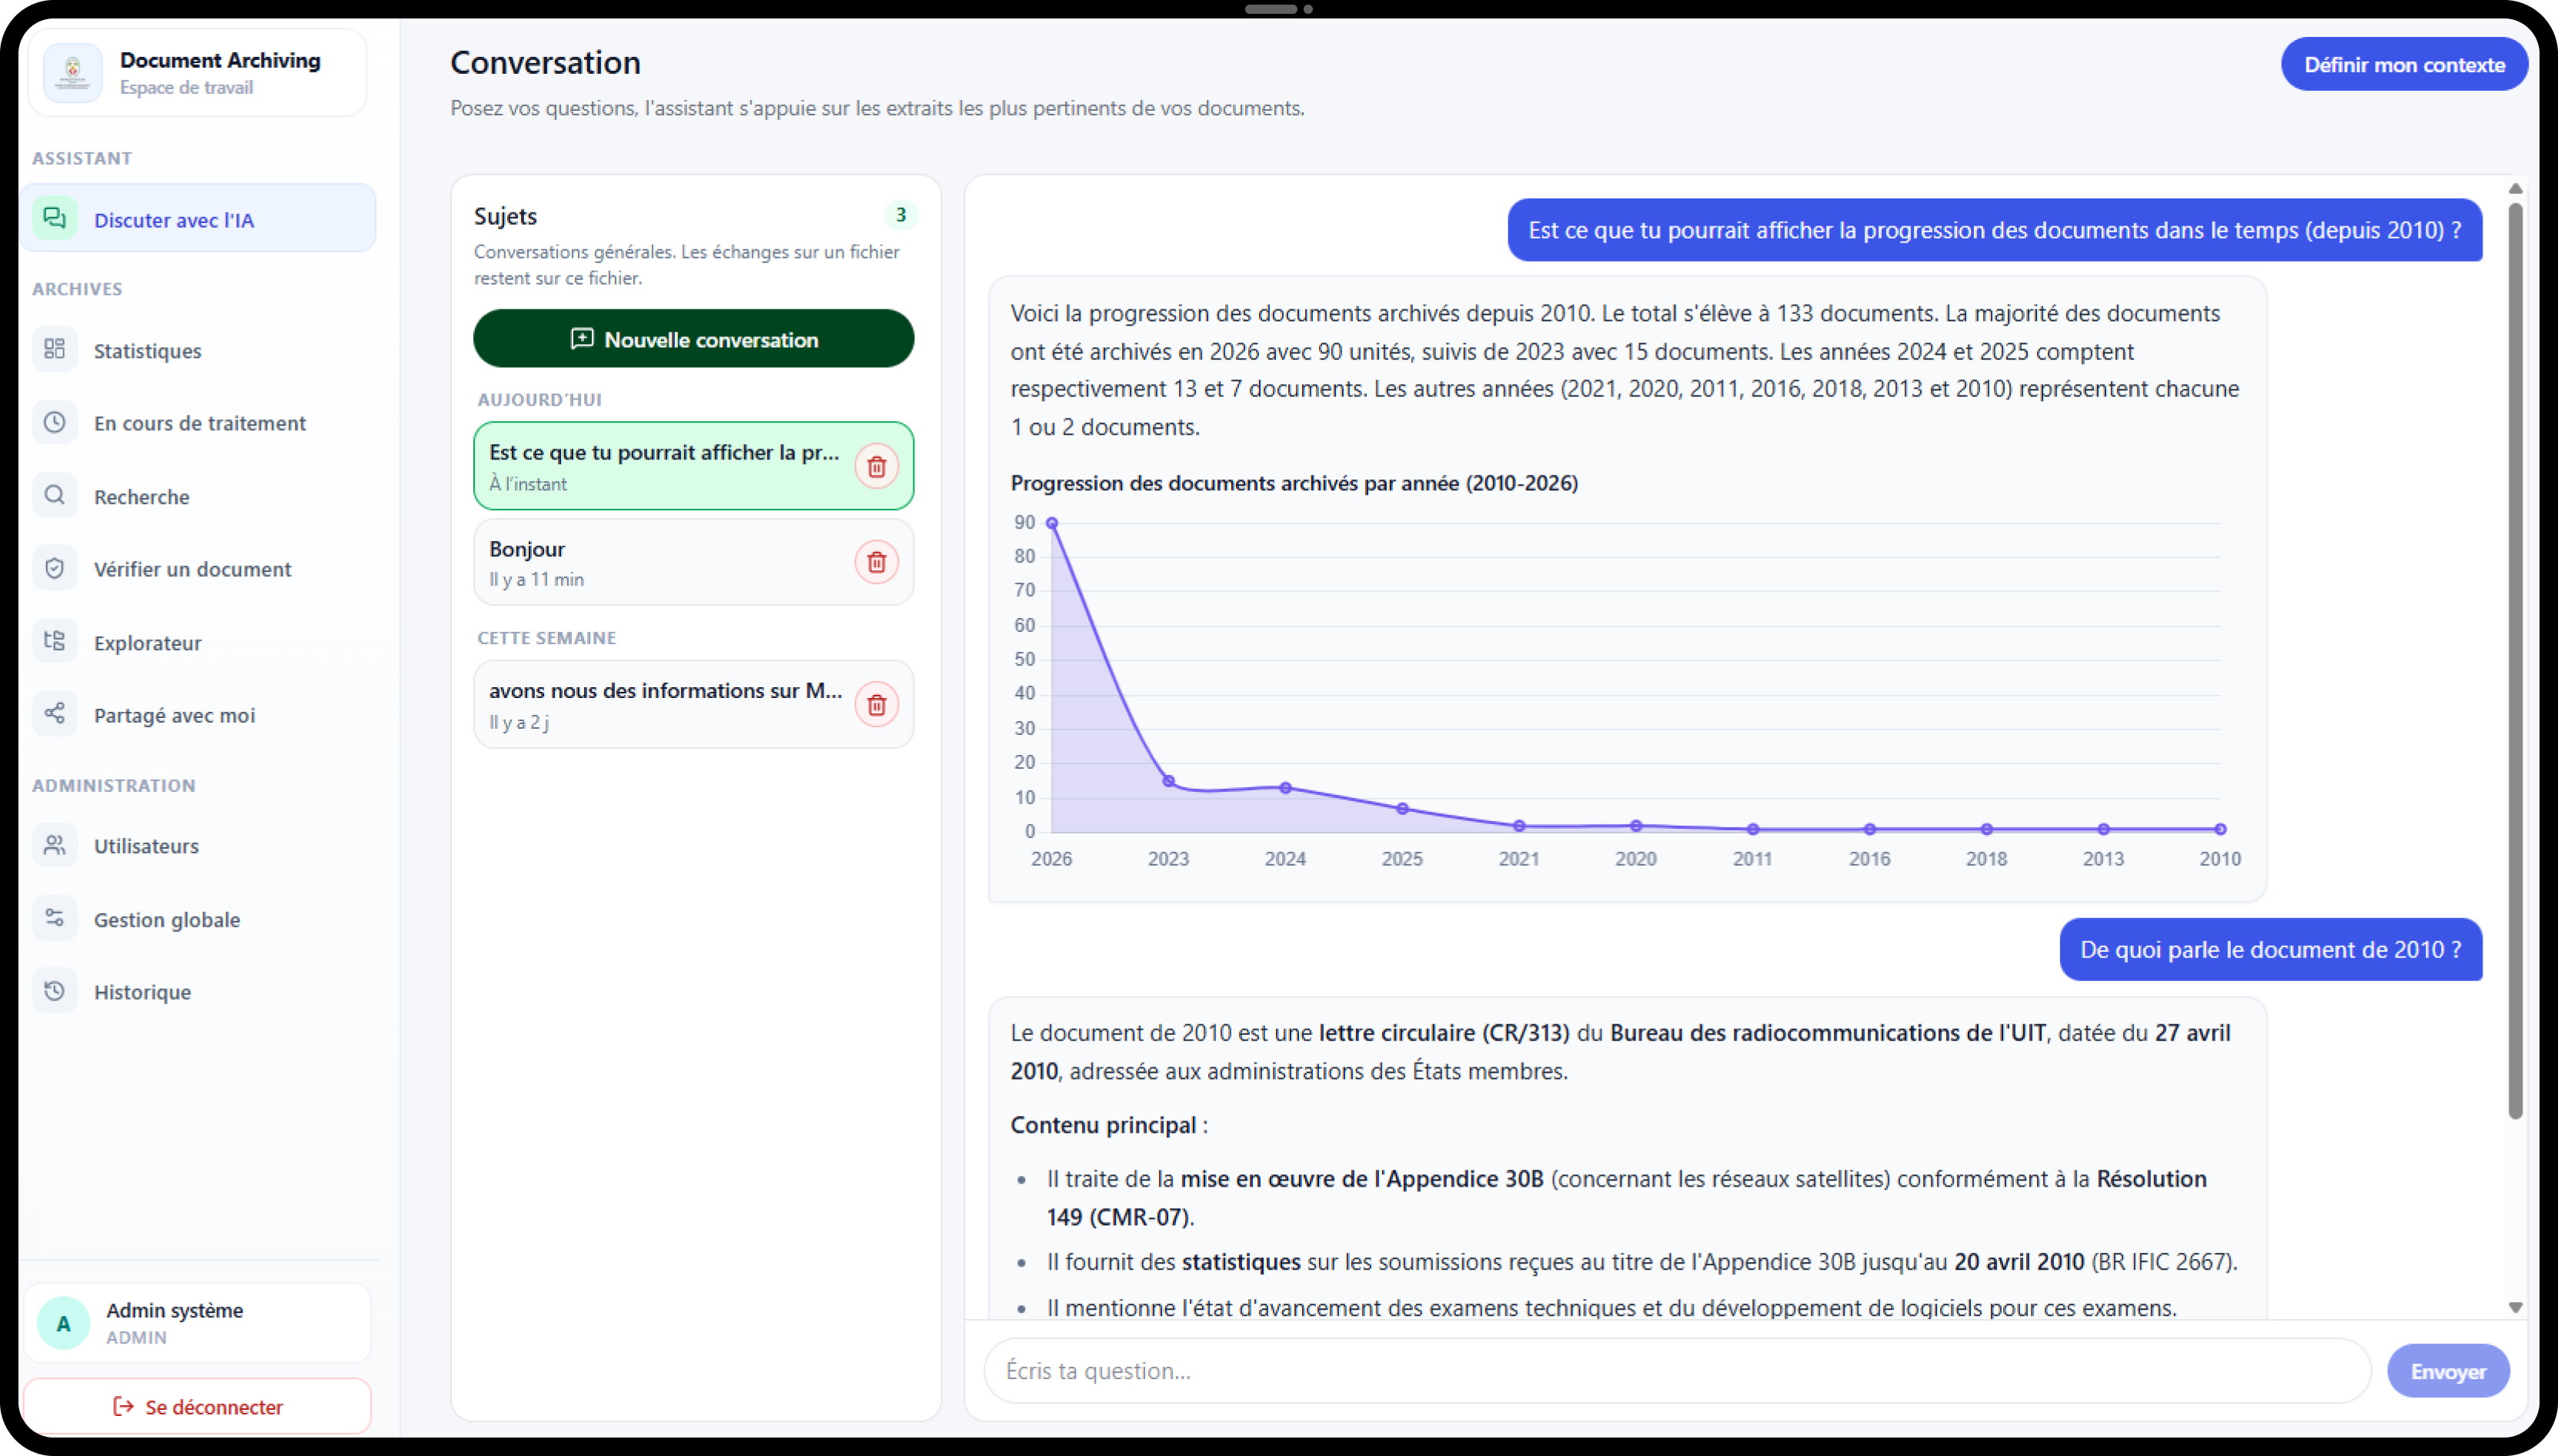
\includegraphics[width=0.98\textwidth]{images/screens/conversation_assistant.png}
\caption{Interface de recherche et d'assistance intelligente}
\label{fig:ui-assistant}
\end{figure}

Enfin, une vue synthétique de l'administration ou du suivi de l'activité illustre les fonctions de gouvernance et de supervision de la plateforme (figure~\ref{fig:ui-dashboard}).

\begin{figure}[H]
\centering
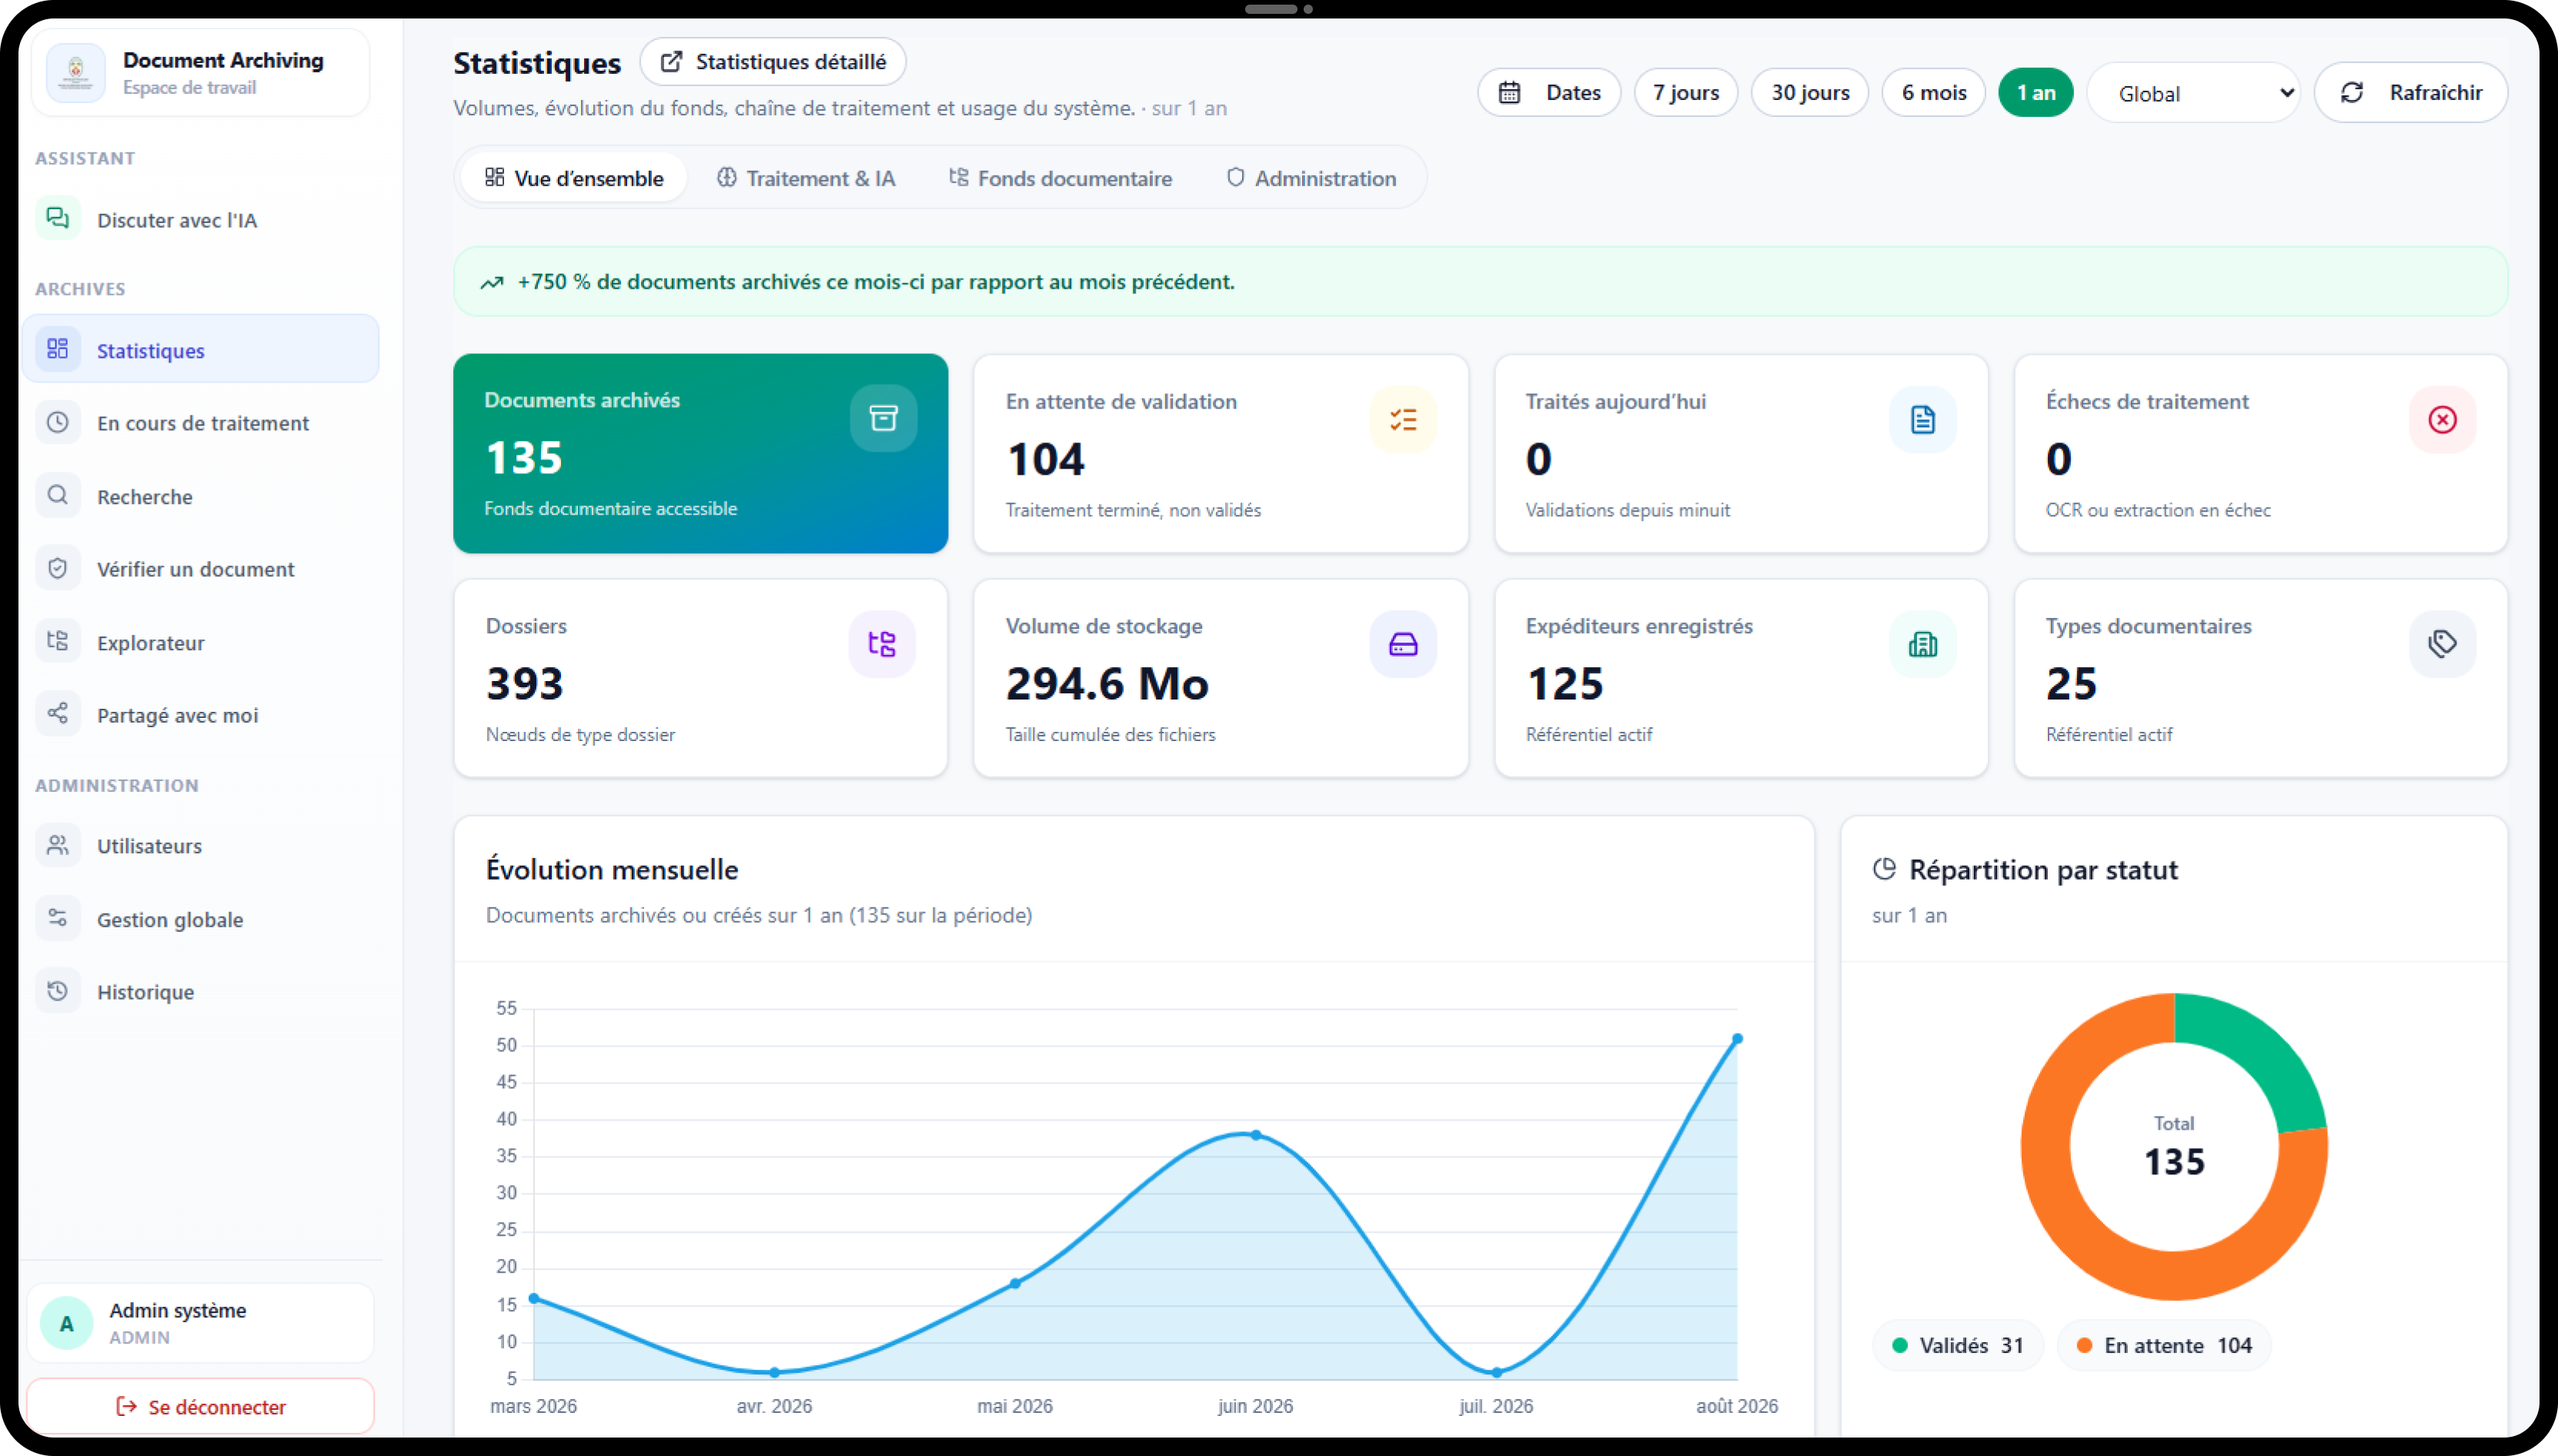
\includegraphics[width=0.98\textwidth]{images/screens/dashboard.png}
\caption{Tableau de bord de supervision de la plateforme}
\label{fig:ui-dashboard}
\end{figure}

Ces parcours traduisent concrètement les choix du chapitre~\ref{ch:conception} : proposer puis valider, classer par règles explicites, rechercher autrement qu'en parcourant l'arbre, et n'afficher que ce que les droits autorisent.

\section{Expérimentations et évaluation}

La conception a volontairement laissé ouverts certains réglages fins, notamment la taille des segments, le nombre d'extraits récupérés, les seuils de similarité et le nombre d'itérations. Cette section confronte ces choix à la solution déployée en environnement interne et revient sur la question posée au chapitre~\ref{ch:existant} : dans les conditions expérimentées, la solution répond-elle aux besoins identifiés ?

L'évaluation ne vise pas à multiplier les indicateurs. Elle les organise autour de quatre dimensions : la qualité du traitement, celle de l'OCR et de l'extraction, celle de la recherche, et celle du RAG. Elle ne constitue pas une preuve statistique généralisable à l'ensemble des archives administratives togolaises. Elle vise à caractériser le fonctionnement de la solution dans les conditions d'exploitation internes, en distinguant ce qui mesure réellement la question posée de ce qui n'en donne que l'apparence.

\subsection{Protocole, corpus et lecture des métriques}

Quatre ensembles doivent être distingués. Le \textbf{fonds historique} du ministère n'est pas mesuré ici dans son intégralité. Le \textbf{flux annuel} est estimé, d'après l'observation du service, à environ 10\,000 dossiers. Le \textbf{fonds accessible en production}, lu sur le tableau de bord le 26~août~2026, compte 35\,007 documents archivés. L'\textbf{échantillon d'évaluation} est un tirage stratifié de 300 documents parmi 34\,917 pièces éligibles (statut technique \texttt{done}, texte OCR ou segments disponibles), avec une graine fixée (\texttt{seed = 42}). Les métriques finales du harnais sont calculées sur le seul split de test ($n = 205$). Les 34\,917 pièces ne remplacent pas le fonds : elles en sont le sous-ensemble éligible au harnais (35\,007 $-$ 34\,917 $=$ 90 documents exclus par le filtre).

Le jeu de données de référence recopie les propositions déjà présentes en production. Les 300 documents ont été marqués comme validés pour le protocole, \textbf{sans relecture humaine des champs ni du texte OCR}. Les scores d'extraction, de type documentaire et d'OCR obtenus contre ce jeu de données de référence comparent donc le système à ses propres sorties. Ils ne sont pas reportés comme résultats : ils ne mesurent pas une performance métier. Les questions de recherche, une par document, ont été générées automatiquement à partir de l'objet et de l'expéditeur ; elles ne constituent pas un jeu métier relu par les agents. Un jeu de données de référence validé par des experts, plus fourni, sur le split de test (type, champs et extrait OCR), est prévu pour une campagne de mesures plus complète ; il n'est pas utilisé dans le présent mémoire.

Le moteur de recherche et l'assistant ont été interrogés en boucle locale sur le serveur de production. Dix objets MinIO de l'échantillon n'ont pas pu être copiés (clé absente ou chemin en base distinct de l'objet réel) ; ces absences limitent un rejeu OCR local, sans empêcher l'évaluation de l'extraction et de la recherche sur le reste du test.

Les paramètres retenus (tableau~\ref{tab:params-rag-realisation}) confirment, en exploitation, les valeurs de conception du tableau~\ref{tab:params-rag-conception} et de l'équation~\eqref{eq:rrf}. Ils ne prétendent pas à un optimum théorique, ni à une généricité hors de ce contexte.

\begin{table}[htbp]
\centering
\caption{Paramètres de travail de la solution déployée (recherche et indexation)}
\label{tab:params-rag-realisation}
\small
\renewcommand{\arraystretch}{1.45}
\begingroup
\rowcolors{2}{black!3}{white}
\begin{tabularx}{\textwidth}{@{}>{\bfseries}Y Y@{}}
\toprule
\rowcolor{black!12}
\tableheader{Paramètre} &
\tableheader{Valeur retenue} \\
\midrule
Taille d'un segment de contenu & environ 2000 caractères \\
Chevauchement & 400 caractères \\
Champs métier exploités & objet, expéditeur, type, destinataire, numéro interne \\
Modèle d'embeddings (local) & MiniLM multilingue, 384 dimensions \\
Fusion & RRF, $k=60$ (non calibré sur le test) \\
Nombre d'extraits (chat) & 8 \\
Statuts du corpus RAG par défaut & VALIDATED (hors DRAFT et corbeille) \\
Passe élargie si vide & implémentée, non isolée dans l'évaluation \\
\bottomrule
\end{tabularx}
\endgroup
\end{table}

\subsection{Qualité du traitement}

Le tableau de bord de production, au 26~août~2026, décrit l'échelle du fonds déjà archivé : 35\,007 documents. Sur ce stock, les trois étapes automatiques (OCR, extraction, analyse par modèle de langage) ont été menées à terme ; 32\,452 pièces sont validées (92,7~\%) et 2\,555 restent en file humaine (7,3~\%). Ces deux effectifs s'ajoutent au fonds : $32\,452 + 2\,555 = 35\,007$. Ce compteur n'est pas un taux d'échec nul du pipeline. En exploitation, sur le flux de traitement, le taux d'échec moyen observé est d'environ 5~\% : texte OCR inexploitable, timeout du modèle de langage, copie objet refusée, fichier isolé dans le répertoire d'erreur, nécessité d'un retraitement. Cette estimation est tirée des journaux Loki des services de traitement et des fichiers isolés dans le répertoire d'erreur du \texttt{scan-listener} ; le dénominateur est le nombre de documents soumis à la chaîne, et non le stock déjà archivé (35\,007) ni l'échantillon du harnais. Le harnais, calculé sur 300 documents déjà en statut \texttt{done}, ne capture pas ces échecs d'entrée ; il décrit la robustesse une fois la chaîne achevée, non le taux d'échec du flux réel.

Ces chiffres mesurent le fonctionnement technique du pipeline, non la justesse des métadonnées. Ils répondent toutefois à un besoin central du chapitre~\ref{ch:existant} : un volume annuel de l'ordre de 10\,000 dossiers ne peut plus reposer sur une saisie unitaire si la chaîne casse trop souvent. Un taux d'échec moyen d'environ 5~\%, avec reprise prévue (répertoire d'erreur, \texttt{reprocess}), reste compatible avec une exploitation interne ; il n'autorise pas à parler d'une chaîne sans défaillance.

Le tableau de bord fournit aussi un \textbf{taux de complétude} des métadonnées, distinct d'un taux de précision. Les propositions de l'IA atteignent une complétude moyenne d'environ 99~\% (100~\% sur les documents déjà validés). Le destinataire est le champ le plus souvent vide côté IA (97,8~\%). Un expéditeur faux mais renseigné compte comme complet : cet indicateur dit seulement si le champ est rempli.

\subsection{Qualité de l'OCR, de la classification et de l'extraction}

Sur le split de test ($n = 205$), le harnais a bien comparé le texte OCR, le type documentaire et les champs extraits aux valeurs déjà stockées en production. Comme le jeu de données de référence recopie ces sorties, le système est comparé à lui-même. Aucun score d'accuracy, de F1 ou de CER/WER n'est donc publié pour cette dimension : un chiffre, même imparfait, y serait lu comme une performance.

Un rejeu Tesseract sur cinq documents, confronté à l'OCR déjà en base, donne un CER moyen de 0,594 et un WER moyen de 0,699. Ce n'est pas un score humain : il mesure l'écart entre un Tesseract local et le texte déjà stocké. Il montre surtout qu'un jeu de données de référence validé par des experts serait nécessaire pour calibrer le moteur. Les temps OCR retenus pour le choix de Tesseract restent des ordres de grandeur observés sur le matériel cible, de l'ordre de 0,8 à 1,5~s par page, et non un engagement de service.

Tant qu'une annotation humaine du test n'est pas disponible, le tableau principal ne porte donc, pour cette dimension, que le temps moyen par page à titre indicatif et la complétude des métadonnées. L'accuracy, le F1 macro, le F1 d'extraction et le CER/WER de qualité n'y figureront qu'après relecture des références.

Les observations de terrain restent utiles pour interpréter ces limites. La qualité de l'OCR paraît liée à celle du scan : un courrier contrasté donne souvent un texte exploitable ; une page sombre, tamponnée ou manuscrite peut produire un OCR pauvre. Le garde-fou heuristique évite de transmettre ce bruit au classifieur. Un repli vers un modèle de vision a, dans certains cas, amélioré la transcription, au prix d'un temps plus élevé. Les erreurs rencontrées lors des essais portent notamment sur des organismes aux libellés proches, une source mal tranchée et des dates ambiguës ; le tableau de bord signale d'ailleurs des millésimes aberrants à nettoyer. Ces cas justifient le maintien de la validation humaine.

\subsection{Qualité de la recherche}

Ce volet est le plus crédible du lot : on compare des identifiants retournés par le service de recherche de production à l'identifiant du document pertinent, et non un champ à lui-même. Les 205 questions du split de test sont toutefois générées automatiquement (objet et expéditeur), ce qui borne l'interprétation.

Le rappel au rang~5 vaut 0,620 : environ 62~\% des questions ramènent le bon document dans les cinq premiers résultats. Le rappel au rang~10 est identique, ce qui indique que, lorsque le document est trouvé dans le haut de liste, il l'est déjà dans le top~5. Le MRR vaut 0,597 : lorsqu'il est trouvé, le document pertinent apparaît en moyenne vers le rang~1. Le nDCG au rang~5 vaut 0,603. Ces trois métriques suffisent pour le tableau principal. La précision aux rangs~5 et~10 (0,124 et 0,062) est mathématiquement cohérente avec un seul document pertinent par requête, mais beaucoup moins intuitive pour le lecteur ; elle n'est pas reprise dans la synthèse.

La latence du moteur, mesurée sur ces 205 requêtes, s'établit à 0,588~s en moyenne et 0,703~s au 95\textsuperscript{e}~percentile. Le maximum (1,342~s) est trop sensible à une requête exceptionnelle pour figurer dans le tableau principal. Pour un service interactif, le p95 sous la seconde est l'indicateur le plus utile.

Ces mesures ne remplacent pas le constat qualitatif déjà formulé lors des essais : une recherche uniquement dense peut manquer un numéro interne, une recherche uniquement lexicale une formulation proche ; la fusion RRF, alimentée aussi par le plein texte et les métadonnées, réduit ces angles morts dans le cadre observé. Huit extraits, avec une limite par document, restent un compromis de configuration, non un optimum démontré.

\subsection{Qualité du RAG}

Le rappel du contexte récupéré, calculé selon le protocole RAGAS \citp{es2024}{Es et al., 2024} sur les 205 questions, vaut 0,838. Il mesure la couverture des passages par rapport à une référence de contexte, et non la \og qualité RAG\fg{} globale. Il ne se confond pas avec le rappel documentaire au rang~5 (0,620) : l'un porte sur des extraits, l'autre sur l'identifiant du document.

La précision de contexte n'a pas pu être calculée (valeur non définie), faute de réponse de référence fournie au juge automatique. Ce n'est pas une métrique de performance ; c'est un état du protocole. De même, une mesure de similarité avec une réponse de référence telle que ROUGE-L \citp{lin2004}{Lin, 2004} et le taux d'ancrage des réponses dans les extraits récupérés (\textit{grounded rate}) n'ont pas été collectés pour ce jeu de 205 questions, bien que l'assistant de production ait été la cible des appels. Ils manquent au tableau principal. Une latence de génération moyenne et au p95 compléterait ce volet ; elle n'est pas reportée ici faute de série transmise.

L'assistant reste donc évalué, à ce stade, par la couverture du contexte récupéré, par les sources affichées dans l'interface, et par la consigne de ne pas compléter une réponse hors extraits. Ce n'est pas encore une mesure de la qualité des réponses générées.

\subsection{Choix des briques OCR et modèle de langage}
\label{sec:eval-choix-briques}

Une comparaison interne a permis de figer le moteur d'OCR et le modèle de langage local. Les temps indiqués sont des ordres de grandeur observés sur le matériel cible, non des engagements de service. Aucune note qualitative par étoiles n'est retenue : le critère déterminant est l'alignement avec un déploiement local, un coût nul à la page, et une latence compatible avec l'usage interactif.

\begin{table}[htbp]
\centering
\caption{Comparaison des moteurs d'OCR examinés (ordres de grandeur)}
\label{tab:choix-ocr}
\small
\renewcommand{\arraystretch}{1.40}
\begingroup
\rowcolors{2}{black!3}{white}
\begin{tabularx}{\textwidth}{@{}>{\bfseries}L{3.4cm}YYY@{}}
\toprule
\rowcolor{black!12}
\tableheader{Solution} &
\tableheader{Temps moyen} &
\tableheader{Déploiement} &
\tableheader{Coût} \\
\midrule
Tesseract~5 & $\sim$0,8--1,5~s/page & local & gratuit \\
EasyOCR & $\sim$3--8~s/page & local & gratuit \\
Moteurs cloud examinés & $\sim$1--4~s/page & distant & payant \\
\bottomrule
\end{tabularx}
\endgroup
\end{table}

Les moteurs cloud examinés (Google Cloud Vision, Azure AI Document Intelligence, AWS Textract) sont en général plus précis sur les scans difficiles, mais imposent un coût à la page, une sortie des documents hors du SI et une dépendance réseau. EasyOCR reste local, au prix d'un débit nettement inférieur pour un gain de précision limité dans le cadre observé. Tesseract~5 a été retenu : local, gratuit, de l'ordre d'une seconde par page, ressources faibles, cohérent avec un fonds de 35\,007 documents. Le rejeu CER/WER sur cinq pages n'invalide pas ce choix ; il rappelle seulement qu'un jeu de données de référence validé par des experts resterait nécessaire pour juger la précision réelle.

\begin{table}[htbp]
\centering
\caption{Comparaison des modèles de langage locaux examinés (Ollama)}
\label{tab:choix-llm}
\small
\renewcommand{\arraystretch}{1.40}
\begingroup
\rowcolors{2}{black!3}{white}
\begin{tabularx}{\textwidth}{@{}>{\bfseries}L{3.6cm}YYYY@{}}
\toprule
\rowcolor{black!12}
\tableheader{Modèle} &
\tableheader{Contexte} &
\tableheader{Temps moyen} &
\tableheader{Ressources} &
\tableheader{Local} \\
\midrule
Llama~3 (8B) & 8K & $\sim$1--3~s & faibles & oui \\
Mistral~7B & 32K & $\sim$2--4~s & faibles & oui \\
GPT-OSS~20B & 128K & $\sim$8--15~s & élevées & oui \\
Qwen3-Coder~30B & 256K & $\sim$17--23~s & élevées & oui \\
\bottomrule
\end{tabularx}
\endgroup
\end{table}

Llama~3 est plus léger, mais le contexte de 8K pèse pour l'extraction et le chat sur dossiers. GPT-OSS et Qwen3-Coder tiennent de plus longs contextes ; un éventuel avantage en raisonnement n'a pas été mesuré dans ce mémoire. Leur latence et leur empreinte mémoire restent, en l'état, incompatibles avec le chat interactif sur le serveur disponible. Mistral~7B tient le compromis retenu : 32K de contexte, quelques secondes par appel, ressources faibles, déploiement entièrement local.

\subsection{Réponse aux besoins du chapitre~\ref{ch:existant}}

Les quatre dimensions se relient aux besoins identifiés après l'analyse de l'existant. Le tableau~\ref{tab:besoins-realisation-ch5}, présenté dans la synthèse du chapitre, rassemble pour chaque besoin la réalisation correspondante et les constats issus de l'évaluation. Le tableau~\ref{tab:eval-systeme} en extrait les métriques conservées dans le résultat principal.

\section{Synthèse}

La conception présentée au chapitre~\ref{ch:conception} a été traduite en une plateforme fonctionnelle déployée en environnement interne. La solution assiste le traitement documentaire depuis l'acquisition jusqu'à la validation humaine, en combinant reconnaissance du contenu, extraction, analyse par intelligence artificielle, proposition de métadonnées, classement déterministe et indexation pour la recherche. Le modèle multi-composante est matérialisé par l'association du stockage objet et de la base de données relationnelle ; le pipeline asynchrone assure l'enchaînement des traitements ; le dispositif de recherche combine plusieurs modes de récupération avant de solliciter le modèle de langage. Les mécanismes de contrôle d'accès, de sensibilité, de journalisation et d'intégrité sont intégrés au fonctionnement de la plateforme.

Le tableau~\ref{tab:eval-systeme} rassemble les métriques dont la lecture est défendable dans l'état actuel du jeu de référence et des logs. Il n'inclut ni les scores d'exactitude obtenus contre les sorties de production, ni la précision au rang~$k$, ni une latence maximale, ni des indicateurs RAG non calculés.

\begin{table}[htbp]
\centering
\caption{Évaluation du système : métriques retenues pour le résultat principal}
\label{tab:eval-systeme}
\small
\renewcommand{\arraystretch}{1.40}
\begingroup
\rowcolors{2}{black!3}{white}
\begin{tabularx}{\textwidth}{@{}L{3.3cm}Y>{\raggedleft\arraybackslash}p{2.7cm}@{}}
\toprule
\rowcolor{black!12}
\tableheader{Dimension} &
\tableheader{Métrique} &
\tableheader{Résultat} \\
\midrule
Robustesse & Documents traités & 35\,007 \\
 & Taux d'échec moyen (exploitation) & $\approx$~5~\% \\
OCR & Temps moyen par page & $\sim$0,8--1,5~s \\
Extraction & Complétude moyenne (propositions IA) & 99~\% \\
Recherche & MRR & 0,597 \\
 & Rappel au rang~5 & 0,620 \\
 & nDCG au rang~5 & 0,603 \\
 & Latence moyenne & 0,588~s \\
 & Latence p95 & 0,703~s \\
RAG & Rappel du contexte récupéré & 0,838 \\
\bottomrule
\end{tabularx}
\endgroup
\end{table}

N'entrent pas dans ce tableau, faute de vérité terrain validée par des experts ou de série transmise : le CER et le WER de qualité, l'accuracy et le F1 macro de classification, le F1 d'extraction, ROUGE-L, le taux d'ancrage des réponses générées, et la latence de l'assistant. Ce n'est pas un vide de protocole : c'est la limite honnête de ce qui peut être affirmé aujourd'hui.

Le tableau~\ref{tab:besoins-realisation-ch5} relie ensuite ces résultats aux besoins du chapitre~\ref{ch:existant}.

\begin{table}[htbp]
\centering
\caption{Besoins identifiés, réalisation et observations issues de l'évaluation}
\label{tab:besoins-realisation-ch5}
\small
\renewcommand{\arraystretch}{1.45}
\begingroup
\rowcolors{2}{black!3}{white}
\begin{tabularx}{\textwidth}{@{}>{\bfseries}Y Y Y@{}}
\toprule
\rowcolor{black!12}
\tableheader{Besoin identifié au chapitre~\ref{ch:existant}} &
\tableheader{Réalisation} &
\tableheader{Observation} \\
\midrule
Réduire le traitement manuel &
Proposition automatique de métadonnées et de classification ; traitement asynchrone &
35\,007 documents traités ; taux d'échec moyen d'environ 5~\% en exploitation ; complétude IA d'environ 99~\% ; une correction humaine reste nécessaire avant validation \\
Fiabiliser le classement &
Construction du chemin à partir des métadonnées validées et de règles déterministes &
Le classement ne dépend pas d'un chemin librement généré par le modèle de langage \\
Conserver le contrôle humain &
États \texttt{DRAFT} et \texttt{VALIDATED} ; validation par un agent &
32\,452 documents validés (92,7~\%) et 2\,555 en file humaine (7,3~\%), soit 35\,007 \\
Faciliter la recherche &
Recherche lexicale, dense et hybride ; RRF ; assistance conversationnelle sourcée &
Rappel au rang~5 de 0,620 et MRR de 0,597 sur 205 questions ; latence p95 de 0,703~s \\
Adapter la structure documentaire &
Référentiels administrables et racines Entrants, Sortants et Internes &
115 types et 13\,244 expéditeurs actifs ; la structure peut être adaptée sans modifier le principe du modèle \\
Sécuriser les archives &
RBAC, ACL, sensibilité, Keycloak et Vault ; filtrage avant récupération &
Le périmètre d'accès est pris en compte avant l'alimentation du contexte destiné au RAG \\
Assurer la traçabilité &
Journalisation des événements, suivi des traitements et empreinte SHA-256 &
Les propositions automatiques peuvent être distinguées des décisions et actions humaines \\
\bottomrule
\end{tabularx}
\endgroup
\end{table}

Au-delà des indicateurs, la solution déployée change le mode de traitement. L'agent n'a plus à renseigner systématiquement l'ensemble des informations avant de classer une pièce : il examine et corrige des propositions. Le classement est ensuite construit à partir des métadonnées retenues et de règles explicites. La recherche interroge le contenu, sous contrainte des droits, avec un rappel au rang~5 de 62~\% sur le jeu automatique du test. Ce n'est pas encore une preuve de qualité des types, des champs ou des réponses générées.

Ces résultats restent limités aux conditions d'exploitation internes et au protocole décrit. Ils ne permettent pas de généraliser un niveau de précision de l'OCR, de la classification ou de l'extraction à l'ensemble des archives administratives togolaises. Le chapitre suivant discute cette portée, les limites du jeu de référence et les perspectives d'une annotation humaine du split de test.
